%%
%% This is file `squelette-rr.tex',
%% generated with the docstrip utility.
%%
%% The original source files were:
%%
%% RR.dtx  (with options: `sample')
%% ********************************************************************
%% Copyright (C) 1997-1999 2004 2006-2011 INRIA/APICS/MARELLE by Jose' Grimm
%% This file may be distributed and/or modified under the
%% conditions of the LaTeX Project Public License, either version 1.3
%% of this license or (at your option) any later version.
%% The latest version of this license is in
%%    http://www.latex-project.org/lppl.txt
%% and version 1.3 or later is part of all distributions of LaTeX
%% version 2003/12/01 or later.
%% An archive of the software can be found at
%%    ftp://ftp-sop.inria.fr/marelle/RR-INRIA
\PassOptionsToPackage{table}{xcolor}
\documentclass[twoside]{article}
\usepackage{etex}
\usepackage[a4paper]{geometry}
\usepackage{RR}
\usepackage{hyperref}

\usepackage{amsmath}
\usepackage{amsthm}
\usepackage{amsfonts}
\usepackage{amssymb}
\usepackage{amsbsy}
\usepackage{stmaryrd} 
\usepackage{subeqnarray}
%%\usepackage[frenchb]{babel} % optionnel
%%\RRNo{7003}
\RTNo{444}
%%
%% date de publication du rapport
\RRdate{\today}
%%
%% Cas d'une version deux
%% \RRversion{2}
%% date de publication de la version 2
%% \RRdater{November 2008}
%%
\RRauthor{% les auteurs
 % Premier auteur, avec une note
Vincent Acary\thanks{INRIA Rh\^one--Alpes. LJK Laboratoire Jean Kuntzman. {\tt vincent.acary@inria.fr}}%
\and
Maurice Br\'emond\thanks{INRIA Rh\^one--Alpes. {\tt maurice.bremond@inria.fr}}%
 % r\'ef\'erence \`a la note partag\'ee
 % liste longue pour tests de mise en page
\and Tomasz Koziara\thanks{School of Engineering and Computing Sciences.Durham University U.K. {\tt tomasz.koziara@durham.ac.uk}} 
\and Franck P\'erignon\thanks{ LJK Laboratoire Jean Kuntzman. {\tt franck.perignon@imag.fr}}}
%% Ceci apparait sur chaque page paire.
\authorhead{Acary \& Br\'emond \& Koziara \& P\'erignon}
%% titre francais long
\RRtitle{FCLIB: une collection de probl\`emes discrets tridimensionels de contact avec frottement}
%% English title
\RRetitle{FCLIB: a collection  of discrete 3D Frictional Contact problems}
%%
\titlehead{FCLIB: a collection  of discrete 3D Frictional Contact  problems}
%%
% \RRnote{This is a note}
% \RRnote{This is a second note}
%%
\RRresume{Le but de ce travail est de mettre en place une collection de probl\`emes discrets de frottement de Coulomb avec contact unilat\'ral. La collection fournira un environnement standard de test pour les algorithmes de r\'esolution, existants et \`a venir. Dans ce document, on d\'ecrit les probl\`emes math\'ematiques que nous voulons collecter et le contenu de la collection courante.
}
\RRabstract{
The goal of this work is to set up a collection of 3D Frictional Contact (3DFC) problems. The collection will provide a standard framework for testing available and new algorithms for solving discrete frictional contact problems. In this document, we describe the mathematical problems that we want to collect and the contents of the current collection. }
%%
\RRmotcle{frottement de Coulomb, contact unilateral, benchmarks}
\RRkeyword{Coulomb's friction, unilateral contact, benchmarks}
%%
%% \RRprojet{Apics}  % cas d'un seul projet
\RRprojet{Bipop}
%%
%% \URLorraine % pour ceux qui sont \`a l'est
%% \URRennes  % pour ceux qui sont \`a l'ouest
%% \URRhoneAlpes % pour ceux qui sont dans les montagnes
%% \URRocq % pour ceux qui sont au centre de la France
%% \URFuturs % pour ceux qui sont dans le virtuel
%% \URSophia % pour ceux qui sont au Sud.
%%
%% \RCBordeaux % centre de recherche Bordeaux - Sud Ouest
%% \RCLille % centre de recherche Lille Nord Europe
%% \RCParis % Paris Rocquencourt
%% \RCSaclay % Saclay \^Ile de France
\RCGrenoble % Grenoble - Rh\^one-Alpes
%% \RCNancy % Nancy - Grand Est
%% \RCRennes % Rennes - Bretagne Atlantique
%%\RCSophia % Sophia Antipolis M\'editerran\'ee

%\input{macro.tex}

\def\n{{\hbox{\tiny{N}}}}
\def\t{{\hbox{\tiny{T}}}}
\newcommand{\RR}{\ensuremath{\rm\sf I\!R}}
\newcommand{\NN}{\ensuremath{\rm\sf I\!N}}


% Packages required by doxygen
\usepackage{calc}
\usepackage{./latex/doxygen}
\usepackage[utf8]{inputenc}
%\usepackage{makeidx}
\usepackage{multicol}
\usepackage{multirow}
\usepackage{textcomp}
\usepackage[table]{xcolor}

% Font selection
\usepackage[T1]{fontenc}
%\usepackage{mathptmx}
%\usepackage[scaled=.90]{helvet}
%\usepackage{courier}
\usepackage{sectsty}
% \renewcommand{\familydefault}{\sfdefault}
% \allsectionsfont{%
%   \fontseries{bc}\selectfont%
%   \color{darkgray}%
% }
\renewcommand{\DoxyLabelFont}{%
  \fontseries{bc}\selectfont%
  \color{darkgray}%
}

% % Page & text layout
% \usepackage{geometry}
% \geometry{%
%   a4paper,%
%   top=2.5cm,%
%   bottom=2.5cm,%
%   left=2.5cm,%
%   right=2.5cm%
% }
% \tolerance=750
% \hfuzz=15pt
% \hbadness=750
% \setlength{\emergencystretch}{15pt}
% \setlength{\parindent}{0cm}
% \setlength{\parskip}{0.2cm}
\makeatletter
% \renewcommand{\paragraph}{%
%   \@startsection{paragraph}{4}{0ex}{-1.0ex}{1.0ex}{%
%     \normalfont\normalsize\bfseries\SS@parafont%
%   }%
% }
\renewcommand{\subparagraph}{%
  \@startsection{subparagraph}{5}{0ex}{-1.0ex}{1.0ex}{%
    \normalfont\normalsize\bfseries\SS@subparafont%
  }%
}
\makeatother
%%

\usepackage{tikz}
\graphicspath{{./figure/},{./latex/}}
\usetikzlibrary{arrows}
\usetikzlibrary{calc}



\begin{document}
%%
%\makeRR   % cas d'un rapport de recherche
\makeRT % cas d'un rapport technique.
%% a partir d'ici, chacun fait comme il le souhaite

\section*{Purpose of the document}



The goal of this work is to set up a collection of 3D Frictional Contact (3DFC) problems. The collection will provide a standard framework for testing available and new algorithms for solving discrete frictional contact problems.  In this document, we describe the mathematical problems that we want to collect and the contents of the current collection.

\section*{Notation}
Let us denote by the integer $n_c$ the number of contacts. The integer $n$ is the number of degree of freedom of the system and $m = 3 n_c$ the number of unknown variables at contacts.

\begin{figure}[htbp]
  \begin{center}

    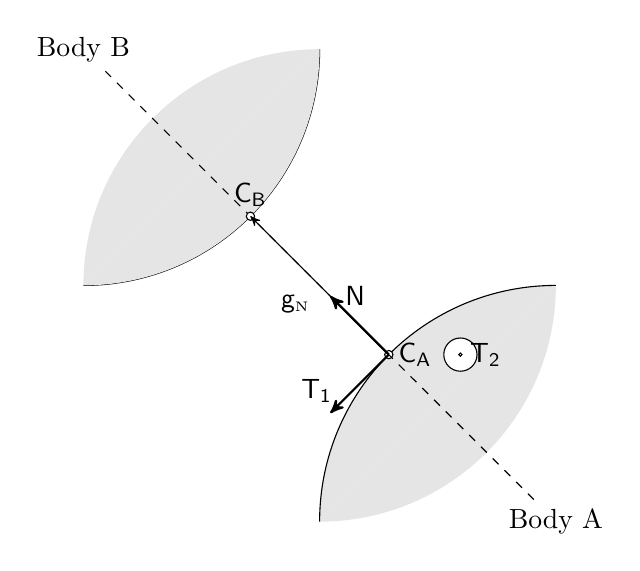
\begin{tikzpicture}[ scale=3,
      axis/.style={ ->, >=stealth'},
      normal/.style={ thick, ->, >=stealth'},
      important line/.style={very thick}, 
      dashed line/.style={dashed, thin},
      every node/.style={color=black},
      soldot/.style={only marks,mark=*},
      holdot/.style={fill=white,only marks,mark=*}
      ]
      % body
      \node (BodyA) at (1,-1) {Body A};
      \fill[gray!20] (1,0) arc (0:-90:1);
      \fill[gray!20] (1,0) arc (90:180:1);
      \draw (1,0) arc (90:180:1);

      \node (BodyB) at (-1,1) {Body B};
      \draw (0,1) arc (0:-90:1);
      \fill[gray!20] (0,1) arc (90:180:1);
      \fill[gray!20] (0,1) arc (0:-90:1);

      % local frame
      \def\nlength{0.35};
      \coordinate (CA)  at  ({1.0-sqrt(2)/2.0},{-1.0+sqrt(2)/2.0});
      \node[] at  (CA) [right] {$\sf C_A$};
      \draw[holdot]  (CA) circle(0.05em);
      \draw[normal] (CA) -- ($(CA)+({-\nlength*sqrt(2)/2.0},{+\nlength*sqrt(2)/2.0 })$) node [right] {$\,\sf N$};
      \draw[normal] (CA) -- ($(CA)+({-\nlength*sqrt(2)/2.0},{-\nlength*sqrt(2)/2.0 })$) node [above] {$\sf T_1\quad$};
      \draw[dashed line] (BodyA) -- (BodyB);
      \draw[holdot] ($(CA)+({\nlength*sqrt(3)/2.0},{0.0})$) circle(0.2em);
      \node at ($(CA)+({\nlength*sqrt(3)/2.0},{0.0})$) [right]{$\sf T_2$};
      \draw[soldot] ($(CA)+({\nlength*sqrt(3)/2.0},{0.0})$) circle(0.02em);
      
      \coordinate (CB)  at  ({-1.0+sqrt(2)/2.0},{1.0-sqrt(2)/2.0});
      \node at  (CB) [above] {$\sf C_B$};
      \draw[holdot]  (CB) circle(0.05em);

      \draw[axis] (CA) -- (CB) node[midway, below left ] {$\sf g_\n$} ;

      % \draw[axis] (0,-0.4) -- (0,0.4) node(yline)[right] {$\sgn(x)$};
      % % lines
      % \draw[important line] (-0.4,-0.3) -- (0.   ,-.3);
      % \draw[important line] (0.0,0.3) --(.4,.3)  ;
      % \coordinate (O) at (0.0, 0.05);
      % \draw[fill] (O) circle (0.03em);
      % \draw (0.0,0.05) node[right]{$a$};
      % \draw (0.0,0.3) node[left]{$1$};
      % \draw (0.0,-0.3) node[right]{$-1$};
      % \draw[holdot] (0.0,0.3) circle (0.03em);
      % \draw[holdot] (0.0,-.3) circle (0.03em);
    \end{tikzpicture}    
  \end{center}
    \caption{Local frame at contact}
    \label{Fig:localframe}
\end{figure}
  
For each contact $\alpha \in \{1,\ldots n_c\}$, the  local velocity  is denoted by $u^\alpha \in \RR^3$. Its normal part  is denoted by $u_\n^{\alpha}\in \RR$ and its tangential part $u_\t\in\RR^2$ (see Figure~\ref{Fig:localframe})
\begin{equation}
  \label{eq:contactvelocity}
  u^\alpha =\left[
  \begin{array}{c}
    u^\alpha_{\n} \\
    u^\alpha_{\t}   
  \end{array}\right].
\end{equation}
The vector $u$ collects all the local velocities at each contact
\begin{equation}
  \label{eq:normal-collect}
  u = [[u^\alpha]^T, \alpha = 1\ldots n_c]^T,
\end{equation}
respectively for the normal part $u_\n$
\begin{equation}
  \label{eq:normal}
  u_\n = [ u^\alpha_{\n}, \alpha = 1\ldots n_c]^T,
\end{equation}
and its tangential a part as 
\begin{equation}
  \label{eq:tangent}
  u_\t = [ [u^\alpha_{\t}]^T, \alpha = 1\ldots n_c]^T.
\end{equation}
For a contact $\alpha $ and a friction coefficient $\mu$, the modified local velocity, denoted by $\hat u^\alpha $, is defined by
\begin{equation}
  \label{eq:modified}
  \hat u^\alpha = u^\alpha +\left[
  \begin{array}{c}
    \mu \|u^\alpha_\t\| \\
    0 \\
    0
  \end{array}\right].
\end{equation}
The vector $\hat u$ collects all the modified local velocity at each contact
\begin{equation}
  \label{eq:normal-modified}
  \hat u = [[\hat u^\alpha]^T, \alpha = 1\ldots n_c]^T.
\end{equation}

For each contact $\alpha$, the reaction vector $r^\alpha\in \RR^3$ is also decomposed in its normal part $r_\n^{\alpha}\in \RR$ and its tangential part $r_\t\in\RR^2$ as
\begin{equation}
  \label{eq:contactreaction}
  r^\alpha = \left[
  \begin{array}{c}
    r^\alpha_{\n} \\
    r^\alpha_{\t}   
  \end{array}\right].
\end{equation}
The Coulomb friction cone for a  contact $\alpha$ is defined by 
\begin{equation}
  \label{eq:CCC}
  K_{\mu^\alpha}^{\alpha}  = \{r^\alpha, \|r^\alpha_\t \| \leq \mu^\alpha |r^\alpha_\n| \}
\end{equation}
and the set $K^{\alpha,\star}_{\mu^\alpha}$ is its dual. The set $K_{\mu}$ is the cartesian product of Coulomb's friction cone at each contact,
\begin{equation}
  \label{eq:CC}
  K_{\mu} = \prod_{\alpha=1\ldots n_c} K_{\mu^\alpha}^{\alpha} 
\end{equation}
For more details, we refer to\cite{Acary.Brogliato2008}.

\clearpage
\section{Linear discrete problems with Coulomb's friction and unilateral contact}
In this section, we formulate basic discrete frictional contact problems considering a finite number $n$ of degrees of freedom  together with a discrete linear dynamics and possibly some bilateral constraints. We assume that a finite set of $n_c$ contact points and their associated local frames has been defined.

\newtheorem{definition}{Definition}

\begin{definition}[Frictional contact problem (3DFC)]\index{mFC3D}
  Given
  \begin{itemize}
    \item a symmetric positive semi--definite  matrix ${W} \in \RR^{m \times m}$
    \item a vector $ {q} \in \RR^m$,
    \item a vector of coefficients of friction $\mu \in \RR^{n_c}$
  \end{itemize}
 the  3DFC problem, denoted by $\mathrm{3DFC}(W,q,\mu)$, consists in finding two vectors $u\in\RR^m$ and $r\in \RR^m$ such that
\begin{equation}\label{eq:3dfc}
  \begin{cases}
    \hat u = W r + q +\left[
      \left[\begin{array}{c}
          \mu^\alpha \|u^\alpha_\t\|\\
          0 \\
          0
        \end{array}\right]^T, \alpha = 1 \ldots n_c
    \right]^T \\ \\
    K^\star_{\mu} \ni {\hat u} \perp r \in K_{\mu}
  \end{cases}
\end{equation}
\qed
\end{definition}

\begin{definition}[Global 3DFrictional contact  problem (G3DFC)]\index{G3DFC}
  Given
  \begin{itemize}
    \item a symmetric positive definite matrix ${M} \in \RR^{n \times n}$
    \item a vector $ {f} \in \RR^n$,
    \item a matrix  ${H} \in \RR^{n \times m}$
    \item a vector $w \in \RR^{m}$,
    \item a vector of coefficients of friction $\mu \in \RR^{n_c}$
  \end{itemize}
 the Global 3DFC problem, denoted by $\mathrm{G3DFC}(M,H,f,w,\mu)$, consists in finding three vectors $ {v} \in \RR^n$, $u\in\RR^m$ and $r\in \RR^m$  such that
\begin{equation}\label{eq:Gfc3d}
  \begin{cases}
    M v = {H} {r} + {f} \\[1mm]
    \hat u = H^T v + w +\left[
      \left[\begin{array}{c}
        \mu^\alpha \|u^\alpha_\t\|\\
        0 \\
        0
      \end{array}\right]^T, \alpha = 1 \ldots n_c
\right]^T \\[1mm]
    K^\star_{\mu} \ni {\hat u} \perp r \in K_{\mu}
  \end{cases}
\end{equation}
\qed
\end{definition}




\begin{definition}[Global  Mixed Frictional contact problem (GM3DFC)]\index{GN3DFC}
  Given
  \begin{itemize}
    \item a symmetric positive definite matrix ${M} \in \RR^{n \times n}$
    \item a vector $ {f} \in \RR^n$,
    \item a matrix  ${H} \in \RR^{n \times m}$
    \item a matrix  ${G} \in \RR^{n \times p}$
     \item a vector $w \in \RR^{m}$,
     \item a vector $b \in \RR^{p}$,
    \item a vector of coefficients of friction $\mu \in \RR^{n_c}$
  \end{itemize}
 the Global Mixed 3DFC problem, denoted by $\mathrm{GM3DFC}(M,H,G,w,b,\mu)$, consists in finding four vectors $ {v} \in \RR^n$, $u\in\RR^m$, $r\in \RR^m$ and $\lambda \in \RR^p$ such that
\begin{equation}\label{eq:gmfc3d}
  \begin{cases}
    M v = {H} {r} + G\lambda + {f} \\[1mm]
    G^T v +b =0 \\[1mm]
    \hat u = H^T v + w +\left[
      \left[\begin{array}{c}
        \mu \|u^\alpha_\t\|\\
        0 \\
        0
      \end{array}\right]^T, \alpha = 1 \ldots n_c
\right]^T \\[1mm]
    K^\star_{\mu} \ni {\hat u} \perp r \in K_{\mu}
  \end{cases}
\end{equation}
\qed
\end{definition}


\begin{definition}[Mixed 3DFrictional contact  problem (M3DFC)]\index{M3DFC}
  Given
  \begin{itemize}
    \item a positive semi--definite matrix  ${W} \in \RR^{m \times m}$
    \item a matrix  ${V} \in \RR^{m \times p}$
    \item a matrix  ${R} \in \RR^{p \times p}$
     \item a vector $q \in \RR^{m}$,
     \item a vector $s \in \RR^{p}$,
    \item a vector of coefficients of friction $\mu \in \RR^{n_c}$
  \end{itemize}
 the  Mixed 3DFC problem, denoted by $\mathrm{M3DFC}(R,V,W,q,s,\mu)$ , consists in finding three vectors $u\in\RR^m$, $r\in \RR^m$ and $\lambda \in \RR^p$  such that
\begin{equation}\label{eq:mfc3d}
  \begin{cases}
    V^T {r} + R \lambda + s = 0 \\[1mm]
    \hat u = W {r}    + V\lambda  + q +\left[
      \left[\begin{array}{c}
        \mu^\alpha \|u^\alpha_\t\|\\
        0 \\
        0
      \end{array}\right]^T, \alpha = 1 \ldots n_c
\right]^T \\[1mm]
   K^\star_{\mu} \ni {\hat u} \perp r \in K_{\mu}
  \end{cases}
\end{equation}
\qed
\end{definition}

\paragraph{Remark}
Note that the previous problems may be an instance of quasi-static problems: the matrix $M$ plays the role of the stiffness matrix and the vector $u$ is a position or a displacement. All the problems can also be an problem in terms of acceleration and forces that we find in event--driven schemes.

%\section{Measuring errors}

\section{Details on the  implementation}

\paragraph{File format}

The proposed file format for storing and managing data is the HDF5 data format\\
 \url{http://www.hdfgroup.org/HDF5}


\noindent The data name should be defined as close as possible to the definition of this document.

\paragraph{Matrix storage}
Several matrix storages are considered :
\begin{enumerate}
\item dense format
\item sparse format : row compressed format, column compressed and triplet (see the description in~\cite{Davis:2006:DMS:1196434}).
\end{enumerate}
The storage of dense matrices is in column major mode (FORTRAN mode). For the sparse matrices, we use the sparse toolkit developed by T. Davis~\cite{Davis:2006:DMS:1196434}.

\paragraph{C implementation}

A C implementation is proposed for reading and writing each of 3DFC problems into HDF5 files. Some details of the C implementation are given in Appendix. More details can be found at \url{http://fclib.gforge.inria.fr}.




\section{Additional  description of the problems}

The following additional information should be added in a reference document and in the HDF5 file.


\begin{itemize}
\item \verb?TITLE? : a title for the problem
\item \verb?DESCRIPTION? : the field of application. Short description on how the problem is generated.
\item \verb?MATRIX_INFO? : the sparsity and the conditioning of the matrices.
\item \verb?MATH_INFO? : existence, uniqueness of solutions.
\item \ldots
\end{itemize}

\noindent The following data can be optionally added in the HDF5 file
\begin{itemize}
\item \verb?SOLUTION? : a reference solution
\item \verb?INITIAL_GUESS? : an initial guess
\item \ldots
\end{itemize}

\clearpage


\section{List of problems in FCLIB.  version 0.2}
\def\ssep{1.5mm}

\begin{itemize}
\item Hanging chain with initial velocity at the tip (see Section~\ref{Sec:Chain}).
\item 100 capsules dropped into a box (see Section~\ref{Sec:Capsules}).
\item 50 boxes stacked under gravity (see Section~\ref{Sec:BoxesStack}).
\item A tower of Kaplas (see Section~\ref{Sec:Kaplas}).
\end{itemize}

For each example, several configurations are available. Each problem is described in a file (HDF5 format) and mainly characterized by the number of degrees of freedom, the number of contacts and the formulation for the contact problem.

\clearpage
\subsection{Hanging chain with initial velocity at the tip.}
\label{Sec:Chain}
{\tt
  \centering
  \begin{tabular}{p{0.3\linewidth}p{0.65\linewidth}}
    \hline \\
    Authors & V. Acary, M. Br\'emond. (INRIA Rh\^one--Alpes) \\
    Date & 10/02/2014\\
    Software & Siconos\\ \\
    \hline \\
  \end{tabular}}

This set of $1514$ problems has been generated by Siconos with the help of Bullet contact detection library. It simulates an hanging chain with initial velocity at the tip. The chain is composed of $11$ elements with the same geometry given by a unique mesh.  The mass of each component is $1$kg for a length of $13.7$m and a thickness of $7.6$m . The initial velocity at the tip is $50$mm/s.

The script that generates this example can be obtained from the Siconos development team. On Figure~\ref{fig:Chain-distrib}, the distribution of the number of contacts, the number of d.o.f and the ratio number of contacts unknowns/number of d.o.f are illustrated.

\begin{minipage}{0.29\linewidth}
  \includegraphics[width=1.0\textwidth]{Chains}
\end{minipage}
\begin{minipage}{0.49\linewidth}
  \begin{tabular}{|p{0.7\textwidth}|c|}
    coefficient of friction & $0.3$ \\[\ssep]
    number of problems & 1514 \\[\ssep]
    number of degrees of freedom & [48:60] \\[\ssep]
    number of contacts & [8:28] \\[\ssep]
    required accuracy   & $10^{-8}$    
  \end{tabular}
\end{minipage}
\begin{figure}[htbp]
  \centering
  \includegraphics[width=0.7\textwidth]{distrib-Chain.pdf}
  \caption{distribution of the number of contacts, the number of d.o.f and their ratio}
  \label{fig:Chain-distrib}
\end{figure}

\clearpage
\subsection{100 capsules dropped into a box.}
\label{Sec:Capsules}
{\tt
  \centering
  \begin{tabular}{p{0.3\linewidth}p{0.65\linewidth}}
    \hline \\
    Authors & V. Acary, M. Br\'emond. (INRIA Rh\^one--Alpes) \\
    Date & 10/02/2014\\
    Software & Siconos\\ \\
    \hline \\
  \end{tabular}}

This set of $1514$ problems has been generated by Siconos with the help of Bullet contact detection library. It simulates $100$ capsules dropped into a box. The Mass of each capsule is $1$kg and length is $5$m. The radius is $1$m.

The script that generates this example can be obtained from the Siconos development team. On Figure~\ref{fig:Capsules-distrib}, the distribution of the number of contacts, the number of d.o.f and the ratio number of contacts unknowns/number of d.o.f are illustrated.

  \begin{minipage}{0.49\linewidth}
    \includegraphics[width=1.0\textwidth]{Capsules}
  \end{minipage}  
  \begin{minipage}{0.49\linewidth}
    \begin{tabular}{|p{0.7\textwidth}|c|}
      coefficient of friction & $0.7$ \\[\ssep]
      number of problems & 1705 \\[\ssep]
      number of degrees of freedom & [6:600] \\[\ssep]
      number of contacts &  [0:300]\\[\ssep]
      required accuracy   & $10^{-8}$    
    \end{tabular}
  \end{minipage}
\begin{figure}[htbp]
  \centering
  
  \includegraphics[width=0.7\textwidth]{distrib-Capsules.pdf}


  \caption{distribution of the number of contacts, the number of d.o.f and their ratio}
  \label{fig:Capsules-distrib}
\end{figure}


\clearpage
\subsection{50 boxes stacked under gravity}
\label{Sec:BoxesStack}
{\tt
  \centering
  \begin{tabular}{p{0.3\linewidth}p{0.65\linewidth}}
    \hline \\
    Authors & V. Acary, M. Br\'emond. (INRIA Rh\^one--Alpes) \\
    Date & 10/02/2014\\
    Software & Siconos\\ \\
    \hline \\
  \end{tabular}}

This set of $1514$ problems has been generated by Siconos with the help of Bullet contact detection library. It simulates 50 boxes stacked under gravity. The mass of the box is $1$kg and the size is $2\times 2$m.
The script that generates this example can be obtained from the Siconos development team. On Figure~\ref{fig:BoxesStack-distrib}, the distribution of the number of contacts, the number of d.o.f and the ratio number of contacts unknowns/number of d.o.f are illustrated.

  \begin{minipage}{0.14\linewidth}
    \includegraphics[width=1.0\textwidth]{BoxesStack}
  \end{minipage}
  \begin{minipage}{0.25\linewidth}
    \includegraphics[width=1.0\textwidth]{BoxesStack2}
  \end{minipage}
  \begin{minipage}{0.49\linewidth}
    \begin{tabular}{|p{0.7\textwidth}|c|}
      coefficient of friction &  0.7\\[\ssep]
      number of problems &  1159 \\[\ssep]
      number of degrees of freedom & [6:300] \\[\ssep]
      number of contacts &  [0:200]\\[\ssep]
      required accuracy   & $10^{-8}$
    \end{tabular}
  \end{minipage}

\begin{figure}[htbp]
  \centering
  
  \includegraphics[width=0.7\textwidth]{distrib-BoxesStack1.pdf}


  \caption{distribution of the number of contacts, the number of d.o.f and their ratio}
  \label{fig:BoxesStack-distrib}
\end{figure}
\clearpage
\subsection{A tower of Kaplas}
\label{Sec:Kaplas}
{\tt
  \centering
  \begin{tabular}{p{0.3\linewidth}p{0.65\linewidth}}
    \hline \\
    Authors & V. Acary, M. Br\'emond. (INRIA Rh\^one--Alpes) \\
    Date & 10/02/2014\\
    Software & Siconos\\ \\
    \hline \\
  \end{tabular}}

This set of $201$ problems has been generated by Siconos with the help of Bullet contact detection library. It simulates a tower of $144$ kaplas of dimension $11.4\times 2.348\times 0.78267$cm. The mass of each is $1$kg. The script that generates this example can be obtained from the Siconos development team. On Figure~\ref{fig:BoxesStack-distrib}, the distribution of the number of contacts, the number of d.o.f and the ratio number of contacts unknowns/number of d.o.f are illustrated.

  \begin{minipage}{0.50\linewidth}
    \includegraphics[width=1.0\textwidth]{KaplasTower}
  \end{minipage}
  \begin{minipage}{0.49\linewidth}
    \begin{tabular}{|p{0.7\textwidth}|c|}
      coefficient of friction &  0.3\\[\ssep]
      number of problems &  201 \\[\ssep]
      number of degrees of freedom & [72:864] \\[\ssep]
      number of contacts &  [0:950]\\[\ssep]
      required accuracy   & $10^{-8}$
    \end{tabular}
  \end{minipage}


\begin{figure}[htbp]
  \centering
  \includegraphics[width=0.7\textwidth]{distrib-KaplasTower.pdf}
  \caption{distribution of the number of contacts, the number of d.o.f and their ratio}
  \label{fig:KaplasTower-distrib}
\end{figure}



\clearpage
\bibliographystyle{plain}
\bibliography{biblio}
\clearpage
\appendix
%--- Begin generated contents ---
% \section{Introduction}
% \label{index}\hypertarget{index}{}\hypertarget{index_whatis}{}\subsection{What is F\-C\-L\-I\-B ?}\label{index_whatis}
F\-C\-L\-I\-B is 
\begin{DoxyItemize}
\item A open source collection of Frictional Contact (F\-C) problems stored in a specific \href{http://www.hdfgroup.org/HDF5/}{\tt H\-D\-F5 format } 
\item A open source light implementation of Input/\-Output functions in C Language to read and write problems  
\end{DoxyItemize}\hypertarget{index_goals}{}\subsection{Goals of the project}\label{index_goals}
The goal of this work is to set up a collection of 2\-D and 3\-D Frictional Contact (F\-C) problems in order to


\begin{DoxyItemize}
\item set up a list of benchmarks  
\item provide a standard framework for testing available and new algorithms for solving discrete frictional contact problems  
\item share common formulations of problems in order to exchange data 
\end{DoxyItemize}\hypertarget{index_howtodownload}{}\subsection{How to download  ?}\label{index_howtodownload}
see \hyperlink{download}{Download} section\hypertarget{index_Wahtis}{}\subsection{What is a Frictional contact problem ?}\label{index_Wahtis}
A Frictional contact problem is algebraic problem obtained after possible time and space discretizations of problems of mechanics of solid involving contact and Coulomb's friction. The mathematical structure of the problem is a second-\/order cone complementarity problem. For more details, you could have a look to the \href{doc/FCLib.pdf}{\tt fclib specifications }\hypertarget{index_Localfclib}{}\subsubsection{The local Frictional Contact problem with equality constraints}\label{index_Localfclib}
Given 
\begin{DoxyItemize}
\item a positive semi--definite matrix ${W} \in {\mathrm{I\!R}}^{m \times m}$ 
\item a matrix ${V} \in {\mathrm{I\!R}}^{m \times p}$ 
\item a matrix ${R} \in {\mathrm{I\!R}}^{p \times p}$ 
\item a vector $q \in {\mathrm{I\!R}}^{m}$, 
\item a vector $s \in {\mathrm{I\!R}}^{p}$, 
\item a vector of coefficients of friction $\mu \in {\mathrm{I\!R}}^{n_c}$ 
\end{DoxyItemize}the Mixed 3\-D\-F\-C problem is to find three vectors $u\in{\mathrm{I\!R}}^m$, $r\in {\mathrm{I\!R}}^m$ and $\lambda \in {\mathrm{I\!R}}^p$ denoted by $\mathrm{M3DFC}(R,V,W,q,s,\mu)$ such that \begin{eqnarray*}\label{eq:lcp1} \begin{cases} V^T {r} + R \lambda + s = 0 \\ \\ \hat u = W {r} + V\lambda + q +\left[ \left[\begin{array}{c} \mu^\alpha \|u^\alpha_T\|\\ 0 \\ 0 \end{array}\right]^T, \alpha = 1 \ldots n_c \right]^T \\ \\ C^\star_{\mu} \ni {\hat u} \perp r \in C_{\mu} \end{cases} \end{eqnarray*} where the Coulomb friction cone for a contact $\alpha$ is defined by \begin{eqnarray*} \label{eq:CCC} C_{\mu^\alpha}^{\alpha} = \{r^\alpha, \|r^\alpha_T \| \leq \mu^\alpha |r^\alpha_N| \} \end{eqnarray*} and the set $C^{\alpha,\star}_{\mu^\alpha}$ is its dual. \hypertarget{index_globalfclib}{}\subsubsection{The Global Frictional Contact problem with equality constraints}\label{index_globalfclib}
We are also dealing with global F\-C problem defined by

Given 
\begin{DoxyItemize}
\item a symmetric positive definite matrix ${M} \in {\mathrm{I\!R}}^{n \times n}$ 
\item a vector $ {f} \in {\mathrm{I\!R}}^n$, 
\item a matrix ${H} \in {\mathrm{I\!R}}^{n \times m}$ 
\item a matrix ${G} \in {\mathrm{I\!R}}^{n \times p}$ 
\item a vector $w \in {\mathrm{I\!R}}^{m}$, 
\item a vector $b \in {\mathrm{I\!R}}^{p}$, 
\item a vector of coefficients of friction $\mu \in {\mathrm{I\!R}}^{n_c}$ 
\end{DoxyItemize}the Global Mixed 3\-D\-F\-C problem is to find four vectors $ {v} \in {\mathrm{I\!R}}^n$, $u\in{\mathrm{I\!R}}^m$, $r\in {\mathrm{I\!R}}^m$ and $\lambda \in {\mathrm{I\!R}}^p$ denoted by $\mathrm{GM3DFC}(M,H,G,w,b,\mu)$ such that \begin{eqnarray*} \begin{cases} M v = {H} {r} + G\lambda + {f} \\ \\ G^T v +b =0 \\ \\ \hat u = H^T v + w +\left[ \left[\begin{array}{c} \mu \|u^\alpha_T\|\\ 0 \\ 0 \end{array}\right]^T, \alpha = 1 \ldots n_c \right]^T \\ \\ C^\star_{\mu} \ni {\hat u} \perp r \in C_{\mu} \end{cases} \end{eqnarray*} \hypertarget{index_wihtout}{}\subsubsection{Problems without equality constraints}\label{index_wihtout}
If the original problems do not contain inequality constraints, or if there are reduced, the problems do no have the variables $\lambda$ as unknowns and can be simplified. However, the storage in H\-D\-F5 file remains the same.\hypertarget{index_Merict}{}\subsubsection{functions.}\label{index_Merict}
The A\-P\-I provides also some Merit functions whixh measures it one set of vectors satifies the previous problems. 
% \section{Download}
% \label{download}
% \hypertarget{download}{}
% \hypertarget{download_howtosources}{}\subsection{How to download sources files of the A\-P\-I?}\label{download_howtosources}

\begin{DoxyItemize}
\item latest version on the svn server access at \href{ https://gforge.inria.fr/scm/?group_id=2824}{\tt F\-C\-L\-I\-B Gforge } 
\item tar files available at \href{https://gforge.inria.fr/frs/?group_id=2824}{\tt F\-C\-L\-I\-B Gforge } 
\end{DoxyItemize}\hypertarget{download_howtolibrary}{}\subsection{How to download the collection of problems ?}\label{download_howtolibrary}

\begin{DoxyItemize}
\item A preliminary version is avalaible here \href{./resources/fclib-library-v0.1.tgz}{\tt F\-C\-L\-I\-B library v 0.\-1 } 
\end{DoxyItemize}\hypertarget{download_howto}{}\subsection{Binaries}\label{download_howto}

\begin{DoxyItemize}
\item Coming soon at \href{https://gforge.inria.fr/frs/?group_id=2824}{\tt F\-C\-L\-I\-B Gforge } 
\end{DoxyItemize}

\par
 \par
 
% \section{Contact us}
% \label{contact}
% \hypertarget{contact}{}
% For any information or help, send an email to  
% \section{Related Publications}
% \label{publications}
% \hypertarget{publications}{}
% \input{./latex/publications}
\section{Class Index}
\subsection{Class List}
Here are the classes, structs, unions and interfaces with brief descriptions\-:\begin{DoxyCompactList}
\item\contentsline{section}{\hyperlink{structcs__dmperm__results}{cs\-\_\-dmperm\-\_\-results} }{\pageref{structcs__dmperm__results}}{}
\item\contentsline{section}{\hyperlink{structcs__numeric}{cs\-\_\-numeric} }{\pageref{structcs__numeric}}{}
\item\contentsline{section}{\hyperlink{structcs__sparse}{cs\-\_\-sparse} }{\pageref{structcs__sparse}}{}
\item\contentsline{section}{\hyperlink{structcs__symbolic}{cs\-\_\-symbolic} }{\pageref{structcs__symbolic}}{}
\item\contentsline{section}{\hyperlink{structfclib__global}{fclib\-\_\-global} \\*The global frictional contact problem defined by }{\pageref{structfclib__global}}{}
\item\contentsline{section}{\hyperlink{structfclib__info}{fclib\-\_\-info} \\*This structure allows the user to enter a problem information as a title, a short description and known mathematical properties of the problem }{\pageref{structfclib__info}}{}
\item\contentsline{section}{\hyperlink{structfclib__local}{fclib\-\_\-local} \\*The local frictional contact problem defined by }{\pageref{structfclib__local}}{}
\item\contentsline{section}{\hyperlink{structfclib__matrix}{fclib\-\_\-matrix} \\*Matrix in compressed row/column or triplet form }{\pageref{structfclib__matrix}}{}
\item\contentsline{section}{\hyperlink{structfclib__matrix__info}{fclib\-\_\-matrix\-\_\-info} \\*This structure allows the user to enter a description for a given matrix (comment, conditionning, determinant, rank.) if they are known }{\pageref{structfclib__matrix__info}}{}
\item\contentsline{section}{\hyperlink{structfclib__solution}{fclib\-\_\-solution} \\*A solution or a guess for the frictional contact problem }{\pageref{structfclib__solution}}{}
\end{DoxyCompactList}

% \section{File Index}
% \subsection{File List}
Here is a list of all files with brief descriptions\-:\begin{DoxyCompactList}
\item\contentsline{section}{\hyperlink{additionalpages_8doxygen}{additionalpages.\-doxygen} }{\pageref{additionalpages_8doxygen}}{}
\item\contentsline{section}{\hyperlink{csparse_8c}{csparse.\-c} }{\pageref{csparse_8c}}{}
\item\contentsline{section}{\hyperlink{csparse_8h}{csparse.\-h} }{\pageref{csparse_8h}}{}
\item\contentsline{section}{\hyperlink{fcint_8h}{fcint.\-h} }{\pageref{fcint_8h}}{}
\item\contentsline{section}{\hyperlink{fclib_8c}{fclib.\-c} }{\pageref{fclib_8c}}{}
\item\contentsline{section}{\hyperlink{fclib_8h}{fclib.\-h} }{\pageref{fclib_8h}}{}
\item\contentsline{section}{\hyperlink{fcmer_8c}{fcmer.\-c} }{\pageref{fcmer_8c}}{}
\item\contentsline{section}{\hyperlink{fctst_8c}{fctst.\-c} }{\pageref{fctst_8c}}{}
\item\contentsline{section}{\hyperlink{fctst__merit_8c}{fctst\-\_\-merit.\-c} }{\pageref{fctst__merit_8c}}{}
\item\contentsline{section}{\hyperlink{mainpage_8doxygen}{mainpage.\-doxygen} }{\pageref{mainpage_8doxygen}}{}
\end{DoxyCompactList}

\section{Class Documentation}
\hypertarget{structcs__dmperm__results}{\subsection{cs\-\_\-dmperm\-\_\-results Struct Reference}
\label{structcs__dmperm__results}\index{cs\-\_\-dmperm\-\_\-results@{cs\-\_\-dmperm\-\_\-results}}
}


{\ttfamily \#include $<$csparse.\-h$>$}

\subsubsection*{Public Attributes}
\begin{DoxyCompactItemize}
\item 
int $\ast$ \hyperlink{structcs__dmperm__results_aaa7aeb656162920573128deddc21f837}{P}
\item 
int $\ast$ \hyperlink{structcs__dmperm__results_a6d15026e4edf9c0e56fbfc7ec758bafb}{Q}
\item 
int $\ast$ \hyperlink{structcs__dmperm__results_a7962d0f1b98b88e96fdc86bfe2be4e39}{R}
\item 
int $\ast$ \hyperlink{structcs__dmperm__results_a841c1955bb06ae973c60fc68b35c9610}{S}
\item 
int \hyperlink{structcs__dmperm__results_a273a6867c52fb2c813575d73ed0d40ee}{nb}
\item 
int \hyperlink{structcs__dmperm__results_af17bae097d2ceb70ca1e8d96006bc225}{rr} \mbox{[}5\mbox{]}
\item 
int \hyperlink{structcs__dmperm__results_ae56ca45f0058903a3c1e586cff63ecef}{cc} \mbox{[}5\mbox{]}
\end{DoxyCompactItemize}


\subsubsection{Detailed Description}


Definition at line 67 of file csparse.\-h.



\subsubsection{Member Data Documentation}
\hypertarget{structcs__dmperm__results_aaa7aeb656162920573128deddc21f837}{\index{cs\-\_\-dmperm\-\_\-results@{cs\-\_\-dmperm\-\_\-results}!P@{P}}
\index{P@{P}!cs_dmperm_results@{cs\-\_\-dmperm\-\_\-results}}
\paragraph[{P}]{\setlength{\rightskip}{0pt plus 5cm}int$\ast$ cs\-\_\-dmperm\-\_\-results\-::\-P}}\label{structcs__dmperm__results_aaa7aeb656162920573128deddc21f837}


Definition at line 69 of file csparse.\-h.



Referenced by cs\-\_\-dalloc(), cs\-\_\-dfree(), cs\-\_\-dmperm(), and cs\-\_\-scc().

\hypertarget{structcs__dmperm__results_a6d15026e4edf9c0e56fbfc7ec758bafb}{\index{cs\-\_\-dmperm\-\_\-results@{cs\-\_\-dmperm\-\_\-results}!Q@{Q}}
\index{Q@{Q}!cs_dmperm_results@{cs\-\_\-dmperm\-\_\-results}}
\paragraph[{Q}]{\setlength{\rightskip}{0pt plus 5cm}int$\ast$ cs\-\_\-dmperm\-\_\-results\-::\-Q}}\label{structcs__dmperm__results_a6d15026e4edf9c0e56fbfc7ec758bafb}


Definition at line 70 of file csparse.\-h.



Referenced by cs\-\_\-dalloc(), cs\-\_\-dfree(), and cs\-\_\-dmperm().

\hypertarget{structcs__dmperm__results_a7962d0f1b98b88e96fdc86bfe2be4e39}{\index{cs\-\_\-dmperm\-\_\-results@{cs\-\_\-dmperm\-\_\-results}!R@{R}}
\index{R@{R}!cs_dmperm_results@{cs\-\_\-dmperm\-\_\-results}}
\paragraph[{R}]{\setlength{\rightskip}{0pt plus 5cm}int$\ast$ cs\-\_\-dmperm\-\_\-results\-::\-R}}\label{structcs__dmperm__results_a7962d0f1b98b88e96fdc86bfe2be4e39}


Definition at line 71 of file csparse.\-h.



Referenced by cs\-\_\-dalloc(), cs\-\_\-dfree(), cs\-\_\-dmperm(), and cs\-\_\-scc().

\hypertarget{structcs__dmperm__results_a841c1955bb06ae973c60fc68b35c9610}{\index{cs\-\_\-dmperm\-\_\-results@{cs\-\_\-dmperm\-\_\-results}!S@{S}}
\index{S@{S}!cs_dmperm_results@{cs\-\_\-dmperm\-\_\-results}}
\paragraph[{S}]{\setlength{\rightskip}{0pt plus 5cm}int$\ast$ cs\-\_\-dmperm\-\_\-results\-::\-S}}\label{structcs__dmperm__results_a841c1955bb06ae973c60fc68b35c9610}


Definition at line 72 of file csparse.\-h.



Referenced by cs\-\_\-dalloc(), cs\-\_\-dfree(), and cs\-\_\-dmperm().

\hypertarget{structcs__dmperm__results_a273a6867c52fb2c813575d73ed0d40ee}{\index{cs\-\_\-dmperm\-\_\-results@{cs\-\_\-dmperm\-\_\-results}!nb@{nb}}
\index{nb@{nb}!cs_dmperm_results@{cs\-\_\-dmperm\-\_\-results}}
\paragraph[{nb}]{\setlength{\rightskip}{0pt plus 5cm}int cs\-\_\-dmperm\-\_\-results\-::nb}}\label{structcs__dmperm__results_a273a6867c52fb2c813575d73ed0d40ee}


Definition at line 73 of file csparse.\-h.



Referenced by cs\-\_\-dmperm(), and cs\-\_\-scc().

\hypertarget{structcs__dmperm__results_af17bae097d2ceb70ca1e8d96006bc225}{\index{cs\-\_\-dmperm\-\_\-results@{cs\-\_\-dmperm\-\_\-results}!rr@{rr}}
\index{rr@{rr}!cs_dmperm_results@{cs\-\_\-dmperm\-\_\-results}}
\paragraph[{rr}]{\setlength{\rightskip}{0pt plus 5cm}int cs\-\_\-dmperm\-\_\-results\-::rr\mbox{[}5\mbox{]}}}\label{structcs__dmperm__results_af17bae097d2ceb70ca1e8d96006bc225}


Definition at line 74 of file csparse.\-h.



Referenced by cs\-\_\-dmperm().

\hypertarget{structcs__dmperm__results_ae56ca45f0058903a3c1e586cff63ecef}{\index{cs\-\_\-dmperm\-\_\-results@{cs\-\_\-dmperm\-\_\-results}!cc@{cc}}
\index{cc@{cc}!cs_dmperm_results@{cs\-\_\-dmperm\-\_\-results}}
\paragraph[{cc}]{\setlength{\rightskip}{0pt plus 5cm}int cs\-\_\-dmperm\-\_\-results\-::cc\mbox{[}5\mbox{]}}}\label{structcs__dmperm__results_ae56ca45f0058903a3c1e586cff63ecef}


Definition at line 75 of file csparse.\-h.



Referenced by cs\-\_\-dmperm().


\hypertarget{structcs__numeric}{\subsection{cs\-\_\-numeric Struct Reference}
\label{structcs__numeric}\index{cs\-\_\-numeric@{cs\-\_\-numeric}}
}


{\ttfamily \#include $<$csparse.\-h$>$}



Collaboration diagram for cs\-\_\-numeric\-:\nopagebreak
\begin{figure}[H]
\begin{center}
\leavevmode
\includegraphics[width=142pt]{structcs__numeric__coll__graph}
\end{center}
\end{figure}
\subsubsection*{Public Attributes}
\begin{DoxyCompactItemize}
\item 
\hyperlink{csparse_8h_a44e471a015cf32e012cffef17e81b6db}{cs} $\ast$ \hyperlink{structcs__numeric_a93a8cf26f01d3df51b41acc690f120d7}{L}
\item 
\hyperlink{csparse_8h_a44e471a015cf32e012cffef17e81b6db}{cs} $\ast$ \hyperlink{structcs__numeric_a1e07204edb10064ca1e471289fced1cb}{U}
\item 
int $\ast$ \hyperlink{structcs__numeric_a485727ef230d7e61b735fad674135d78}{Pinv}
\item 
double $\ast$ \hyperlink{structcs__numeric_ad81bc354670c58c7e715293e98316152}{B}
\end{DoxyCompactItemize}


\subsubsection{Detailed Description}


Definition at line 59 of file csparse.\-h.



\subsubsection{Member Data Documentation}
\hypertarget{structcs__numeric_a93a8cf26f01d3df51b41acc690f120d7}{\index{cs\-\_\-numeric@{cs\-\_\-numeric}!L@{L}}
\index{L@{L}!cs_numeric@{cs\-\_\-numeric}}
\paragraph[{L}]{\setlength{\rightskip}{0pt plus 5cm}{\bf cs}$\ast$ cs\-\_\-numeric\-::\-L}}\label{structcs__numeric_a93a8cf26f01d3df51b41acc690f120d7}


Definition at line 61 of file csparse.\-h.



Referenced by cs\-\_\-chol(), cs\-\_\-cholsol(), cs\-\_\-lu(), cs\-\_\-lusol(), cs\-\_\-nfree(), cs\-\_\-qr(), and cs\-\_\-qrsol().

\hypertarget{structcs__numeric_a1e07204edb10064ca1e471289fced1cb}{\index{cs\-\_\-numeric@{cs\-\_\-numeric}!U@{U}}
\index{U@{U}!cs_numeric@{cs\-\_\-numeric}}
\paragraph[{U}]{\setlength{\rightskip}{0pt plus 5cm}{\bf cs}$\ast$ cs\-\_\-numeric\-::\-U}}\label{structcs__numeric_a1e07204edb10064ca1e471289fced1cb}


Definition at line 62 of file csparse.\-h.



Referenced by cs\-\_\-lu(), cs\-\_\-lusol(), cs\-\_\-nfree(), cs\-\_\-qr(), and cs\-\_\-qrsol().

\hypertarget{structcs__numeric_a485727ef230d7e61b735fad674135d78}{\index{cs\-\_\-numeric@{cs\-\_\-numeric}!Pinv@{Pinv}}
\index{Pinv@{Pinv}!cs_numeric@{cs\-\_\-numeric}}
\paragraph[{Pinv}]{\setlength{\rightskip}{0pt plus 5cm}int$\ast$ cs\-\_\-numeric\-::\-Pinv}}\label{structcs__numeric_a485727ef230d7e61b735fad674135d78}


Definition at line 63 of file csparse.\-h.



Referenced by cs\-\_\-lu(), cs\-\_\-lusol(), and cs\-\_\-nfree().

\hypertarget{structcs__numeric_ad81bc354670c58c7e715293e98316152}{\index{cs\-\_\-numeric@{cs\-\_\-numeric}!B@{B}}
\index{B@{B}!cs_numeric@{cs\-\_\-numeric}}
\paragraph[{B}]{\setlength{\rightskip}{0pt plus 5cm}double$\ast$ cs\-\_\-numeric\-::\-B}}\label{structcs__numeric_ad81bc354670c58c7e715293e98316152}


Definition at line 64 of file csparse.\-h.



Referenced by cs\-\_\-nfree(), cs\-\_\-qr(), and cs\-\_\-qrsol().


\hypertarget{structcs__sparse}{\subsection{cs\-\_\-sparse Struct Reference}
\label{structcs__sparse}\index{cs\-\_\-sparse@{cs\-\_\-sparse}}
}


{\ttfamily \#include $<$csparse.\-h$>$}

\subsubsection*{Public Attributes}
\begin{DoxyCompactItemize}
\item 
int \hyperlink{structcs__sparse_aab49fc365ddf6273376a96d3a6aa751f}{nzmax}
\item 
int \hyperlink{structcs__sparse_a8aeba3ffed4d599a4906e78329d3448b}{m}
\item 
int \hyperlink{structcs__sparse_a86c18870dc1551c71f8ea551efe68625}{n}
\item 
int $\ast$ \hyperlink{structcs__sparse_a263a2347e8dcf1a7a20ee66730297b85}{p}
\item 
int $\ast$ \hyperlink{structcs__sparse_aeb6831b93f8a901b4a5d520c46990f44}{i}
\item 
double $\ast$ \hyperlink{structcs__sparse_a0d6d06e4893a7d4d86e94ce49358d9c1}{x}
\item 
int \hyperlink{structcs__sparse_a707363d7869d3fc4126027c1c9c7cf7c}{nz}
\end{DoxyCompactItemize}


\subsubsection{Detailed Description}


Definition at line 14 of file csparse.\-h.



\subsubsection{Member Data Documentation}
\hypertarget{structcs__sparse_aab49fc365ddf6273376a96d3a6aa751f}{\index{cs\-\_\-sparse@{cs\-\_\-sparse}!nzmax@{nzmax}}
\index{nzmax@{nzmax}!cs_sparse@{cs\-\_\-sparse}}
\paragraph[{nzmax}]{\setlength{\rightskip}{0pt plus 5cm}int cs\-\_\-sparse\-::nzmax}}\label{structcs__sparse_aab49fc365ddf6273376a96d3a6aa751f}


Definition at line 16 of file csparse.\-h.



Referenced by cs\-\_\-amd(), cs\-\_\-entry(), cs\-\_\-lu(), cs\-\_\-print(), cs\-\_\-spalloc(), and cs\-\_\-sprealloc().

\hypertarget{structcs__sparse_a8aeba3ffed4d599a4906e78329d3448b}{\index{cs\-\_\-sparse@{cs\-\_\-sparse}!m@{m}}
\index{m@{m}!cs_sparse@{cs\-\_\-sparse}}
\paragraph[{m}]{\setlength{\rightskip}{0pt plus 5cm}int cs\-\_\-sparse\-::m}}\label{structcs__sparse_a8aeba3ffed4d599a4906e78329d3448b}


Definition at line 17 of file csparse.\-h.



Referenced by cs\-\_\-add(), cs\-\_\-amd(), cs\-\_\-counts(), cs\-\_\-dmperm(), cs\-\_\-dupl(), cs\-\_\-entry(), cs\-\_\-etree(), cs\-\_\-maxtrans(), cs\-\_\-multiply(), cs\-\_\-permute(), cs\-\_\-print(), cs\-\_\-qr(), cs\-\_\-qrsol(), cs\-\_\-spalloc(), cs\-\_\-transpose(), cs\-\_\-triplet(), and cs\-\_\-vcount().

\hypertarget{structcs__sparse_a86c18870dc1551c71f8ea551efe68625}{\index{cs\-\_\-sparse@{cs\-\_\-sparse}!n@{n}}
\index{n@{n}!cs_sparse@{cs\-\_\-sparse}}
\paragraph[{n}]{\setlength{\rightskip}{0pt plus 5cm}int cs\-\_\-sparse\-::n}}\label{structcs__sparse_a86c18870dc1551c71f8ea551efe68625}


Definition at line 18 of file csparse.\-h.



Referenced by cs\-\_\-add(), cs\-\_\-amd(), cs\-\_\-chol(), cs\-\_\-cholsol(), cs\-\_\-counts(), cs\-\_\-dmperm(), cs\-\_\-dupl(), cs\-\_\-entry(), cs\-\_\-etree(), cs\-\_\-fkeep(), cs\-\_\-gaxpy(), cs\-\_\-lsolve(), cs\-\_\-ltsolve(), cs\-\_\-lu(), cs\-\_\-lusol(), cs\-\_\-maxtrans(), cs\-\_\-multiply(), cs\-\_\-norm(), cs\-\_\-permute(), cs\-\_\-print(), cs\-\_\-qr(), cs\-\_\-qrsol(), cs\-\_\-reach(), cs\-\_\-scc(), cs\-\_\-schol(), cs\-\_\-spalloc(), cs\-\_\-splsolve(), cs\-\_\-sprealloc(), cs\-\_\-sqr(), cs\-\_\-symperm(), cs\-\_\-transpose(), cs\-\_\-triplet(), cs\-\_\-updown(), cs\-\_\-usolve(), cs\-\_\-utsolve(), and cs\-\_\-vcount().

\hypertarget{structcs__sparse_a263a2347e8dcf1a7a20ee66730297b85}{\index{cs\-\_\-sparse@{cs\-\_\-sparse}!p@{p}}
\index{p@{p}!cs_sparse@{cs\-\_\-sparse}}
\paragraph[{p}]{\setlength{\rightskip}{0pt plus 5cm}int$\ast$ cs\-\_\-sparse\-::p}}\label{structcs__sparse_a263a2347e8dcf1a7a20ee66730297b85}


Definition at line 19 of file csparse.\-h.



Referenced by cs\-\_\-add(), cs\-\_\-amd(), cs\-\_\-augment(), cs\-\_\-bfs(), cs\-\_\-chol(), cs\-\_\-counts(), cs\-\_\-dfs(), cs\-\_\-dmperm(), cs\-\_\-dupl(), cs\-\_\-entry(), cs\-\_\-ereach(), cs\-\_\-etree(), cs\-\_\-fkeep(), cs\-\_\-gaxpy(), cs\-\_\-happly(), cs\-\_\-lsolve(), cs\-\_\-ltsolve(), cs\-\_\-lu(), cs\-\_\-maxtrans(), cs\-\_\-multiply(), cs\-\_\-norm(), cs\-\_\-permute(), cs\-\_\-print(), cs\-\_\-qr(), cs\-\_\-reach(), cs\-\_\-scatter(), cs\-\_\-scc(), cs\-\_\-spalloc(), cs\-\_\-spfree(), cs\-\_\-splsolve(), cs\-\_\-sprealloc(), cs\-\_\-sqr(), cs\-\_\-symperm(), cs\-\_\-transpose(), cs\-\_\-triplet(), cs\-\_\-updown(), cs\-\_\-usolve(), cs\-\_\-utsolve(), and cs\-\_\-vcount().

\hypertarget{structcs__sparse_aeb6831b93f8a901b4a5d520c46990f44}{\index{cs\-\_\-sparse@{cs\-\_\-sparse}!i@{i}}
\index{i@{i}!cs_sparse@{cs\-\_\-sparse}}
\paragraph[{i}]{\setlength{\rightskip}{0pt plus 5cm}int$\ast$ cs\-\_\-sparse\-::i}}\label{structcs__sparse_aeb6831b93f8a901b4a5d520c46990f44}


Definition at line 20 of file csparse.\-h.



Referenced by cs\-\_\-amd(), cs\-\_\-augment(), cs\-\_\-bfs(), cs\-\_\-chol(), cs\-\_\-counts(), cs\-\_\-dfs(), cs\-\_\-dmperm(), cs\-\_\-dupl(), cs\-\_\-entry(), cs\-\_\-ereach(), cs\-\_\-etree(), cs\-\_\-fkeep(), cs\-\_\-gaxpy(), cs\-\_\-happly(), cs\-\_\-lsolve(), cs\-\_\-ltsolve(), cs\-\_\-lu(), cs\-\_\-maxtrans(), cs\-\_\-multiply(), cs\-\_\-permute(), cs\-\_\-print(), cs\-\_\-qr(), cs\-\_\-reach(), cs\-\_\-scatter(), cs\-\_\-spalloc(), cs\-\_\-spfree(), cs\-\_\-splsolve(), cs\-\_\-sprealloc(), cs\-\_\-symperm(), cs\-\_\-transpose(), cs\-\_\-triplet(), cs\-\_\-updown(), cs\-\_\-usolve(), cs\-\_\-utsolve(), and cs\-\_\-vcount().

\hypertarget{structcs__sparse_a0d6d06e4893a7d4d86e94ce49358d9c1}{\index{cs\-\_\-sparse@{cs\-\_\-sparse}!x@{x}}
\index{x@{x}!cs_sparse@{cs\-\_\-sparse}}
\paragraph[{x}]{\setlength{\rightskip}{0pt plus 5cm}double$\ast$ cs\-\_\-sparse\-::x}}\label{structcs__sparse_a0d6d06e4893a7d4d86e94ce49358d9c1}


Definition at line 21 of file csparse.\-h.



Referenced by cs\-\_\-add(), cs\-\_\-chol(), cs\-\_\-dupl(), cs\-\_\-entry(), cs\-\_\-ereach(), cs\-\_\-fkeep(), cs\-\_\-gaxpy(), cs\-\_\-happly(), cs\-\_\-lsolve(), cs\-\_\-ltsolve(), cs\-\_\-lu(), cs\-\_\-multiply(), cs\-\_\-norm(), cs\-\_\-permute(), cs\-\_\-print(), cs\-\_\-qr(), cs\-\_\-scatter(), cs\-\_\-spalloc(), cs\-\_\-spfree(), cs\-\_\-splsolve(), cs\-\_\-sprealloc(), cs\-\_\-symperm(), cs\-\_\-transpose(), cs\-\_\-triplet(), cs\-\_\-updown(), cs\-\_\-usolve(), and cs\-\_\-utsolve().

\hypertarget{structcs__sparse_a707363d7869d3fc4126027c1c9c7cf7c}{\index{cs\-\_\-sparse@{cs\-\_\-sparse}!nz@{nz}}
\index{nz@{nz}!cs_sparse@{cs\-\_\-sparse}}
\paragraph[{nz}]{\setlength{\rightskip}{0pt plus 5cm}int cs\-\_\-sparse\-::nz}}\label{structcs__sparse_a707363d7869d3fc4126027c1c9c7cf7c}


Definition at line 22 of file csparse.\-h.



Referenced by cs\-\_\-entry(), cs\-\_\-print(), cs\-\_\-spalloc(), cs\-\_\-sprealloc(), and cs\-\_\-triplet().


\hypertarget{structcs__symbolic}{\subsection{cs\-\_\-symbolic Struct Reference}
\label{structcs__symbolic}\index{cs\-\_\-symbolic@{cs\-\_\-symbolic}}
}


{\ttfamily \#include $<$csparse.\-h$>$}

\subsubsection*{Public Attributes}
\begin{DoxyCompactItemize}
\item 
int $\ast$ \hyperlink{structcs__symbolic_a095ba468af8cb63c4cecf46a1adb45ac}{Pinv}
\item 
int $\ast$ \hyperlink{structcs__symbolic_afcefa00ab98cf91d2258dc5a63f7dd6d}{Q}
\item 
int $\ast$ \hyperlink{structcs__symbolic_aefc6fc6ae59f5c51b225c93a549b6838}{parent}
\item 
int $\ast$ \hyperlink{structcs__symbolic_a85eed6fd134282ada142ebaae0fe2403}{cp}
\item 
int \hyperlink{structcs__symbolic_a6e76dde6232a98e3b5d96d942c08b12e}{m2}
\item 
int \hyperlink{structcs__symbolic_acfb8969ebae172c2efcc82e1b98ef826}{lnz}
\item 
int \hyperlink{structcs__symbolic_ad20740ef6e60d2a90e12860c0bf6aab7}{unz}
\end{DoxyCompactItemize}


\subsubsection{Detailed Description}


Definition at line 48 of file csparse.\-h.



\subsubsection{Member Data Documentation}
\hypertarget{structcs__symbolic_a095ba468af8cb63c4cecf46a1adb45ac}{\index{cs\-\_\-symbolic@{cs\-\_\-symbolic}!Pinv@{Pinv}}
\index{Pinv@{Pinv}!cs_symbolic@{cs\-\_\-symbolic}}
\paragraph[{Pinv}]{\setlength{\rightskip}{0pt plus 5cm}int$\ast$ cs\-\_\-symbolic\-::\-Pinv}}\label{structcs__symbolic_a095ba468af8cb63c4cecf46a1adb45ac}


Definition at line 50 of file csparse.\-h.



Referenced by cs\-\_\-chol(), cs\-\_\-cholsol(), cs\-\_\-qr(), cs\-\_\-qrsol(), cs\-\_\-schol(), cs\-\_\-sfree(), and cs\-\_\-sqr().

\hypertarget{structcs__symbolic_afcefa00ab98cf91d2258dc5a63f7dd6d}{\index{cs\-\_\-symbolic@{cs\-\_\-symbolic}!Q@{Q}}
\index{Q@{Q}!cs_symbolic@{cs\-\_\-symbolic}}
\paragraph[{Q}]{\setlength{\rightskip}{0pt plus 5cm}int$\ast$ cs\-\_\-symbolic\-::\-Q}}\label{structcs__symbolic_afcefa00ab98cf91d2258dc5a63f7dd6d}


Definition at line 51 of file csparse.\-h.



Referenced by cs\-\_\-lu(), cs\-\_\-lusol(), cs\-\_\-qr(), cs\-\_\-qrsol(), cs\-\_\-sfree(), and cs\-\_\-sqr().

\hypertarget{structcs__symbolic_aefc6fc6ae59f5c51b225c93a549b6838}{\index{cs\-\_\-symbolic@{cs\-\_\-symbolic}!parent@{parent}}
\index{parent@{parent}!cs_symbolic@{cs\-\_\-symbolic}}
\paragraph[{parent}]{\setlength{\rightskip}{0pt plus 5cm}int$\ast$ cs\-\_\-symbolic\-::parent}}\label{structcs__symbolic_aefc6fc6ae59f5c51b225c93a549b6838}


Definition at line 52 of file csparse.\-h.



Referenced by cs\-\_\-chol(), cs\-\_\-qr(), cs\-\_\-schol(), cs\-\_\-sfree(), and cs\-\_\-sqr().

\hypertarget{structcs__symbolic_a85eed6fd134282ada142ebaae0fe2403}{\index{cs\-\_\-symbolic@{cs\-\_\-symbolic}!cp@{cp}}
\index{cp@{cp}!cs_symbolic@{cs\-\_\-symbolic}}
\paragraph[{cp}]{\setlength{\rightskip}{0pt plus 5cm}int$\ast$ cs\-\_\-symbolic\-::cp}}\label{structcs__symbolic_a85eed6fd134282ada142ebaae0fe2403}


Definition at line 53 of file csparse.\-h.



Referenced by cs\-\_\-chol(), cs\-\_\-schol(), cs\-\_\-sfree(), and cs\-\_\-sqr().

\hypertarget{structcs__symbolic_a6e76dde6232a98e3b5d96d942c08b12e}{\index{cs\-\_\-symbolic@{cs\-\_\-symbolic}!m2@{m2}}
\index{m2@{m2}!cs_symbolic@{cs\-\_\-symbolic}}
\paragraph[{m2}]{\setlength{\rightskip}{0pt plus 5cm}int cs\-\_\-symbolic\-::m2}}\label{structcs__symbolic_a6e76dde6232a98e3b5d96d942c08b12e}


Definition at line 54 of file csparse.\-h.



Referenced by cs\-\_\-qr(), cs\-\_\-qrsol(), and cs\-\_\-sqr().

\hypertarget{structcs__symbolic_acfb8969ebae172c2efcc82e1b98ef826}{\index{cs\-\_\-symbolic@{cs\-\_\-symbolic}!lnz@{lnz}}
\index{lnz@{lnz}!cs_symbolic@{cs\-\_\-symbolic}}
\paragraph[{lnz}]{\setlength{\rightskip}{0pt plus 5cm}int cs\-\_\-symbolic\-::lnz}}\label{structcs__symbolic_acfb8969ebae172c2efcc82e1b98ef826}


Definition at line 55 of file csparse.\-h.



Referenced by cs\-\_\-lu(), cs\-\_\-qr(), cs\-\_\-schol(), and cs\-\_\-sqr().

\hypertarget{structcs__symbolic_ad20740ef6e60d2a90e12860c0bf6aab7}{\index{cs\-\_\-symbolic@{cs\-\_\-symbolic}!unz@{unz}}
\index{unz@{unz}!cs_symbolic@{cs\-\_\-symbolic}}
\paragraph[{unz}]{\setlength{\rightskip}{0pt plus 5cm}int cs\-\_\-symbolic\-::unz}}\label{structcs__symbolic_ad20740ef6e60d2a90e12860c0bf6aab7}


Definition at line 56 of file csparse.\-h.



Referenced by cs\-\_\-lu(), cs\-\_\-qr(), cs\-\_\-schol(), and cs\-\_\-sqr().


\hypertarget{structfclib__global}{\subsection{fclib\-\_\-global Struct Reference}
\label{structfclib__global}\index{fclib\-\_\-global@{fclib\-\_\-global}}
}


The global frictional contact problem defined by.  




{\ttfamily \#include $<$fclib.\-h$>$}



Collaboration diagram for fclib\-\_\-global\-:\nopagebreak
\begin{figure}[H]
\begin{center}
\leavevmode
\includegraphics[width=222pt]{structfclib__global__coll__graph}
\end{center}
\end{figure}
\subsubsection*{Public Attributes}
\begin{DoxyCompactItemize}
\item 
struct \hyperlink{structfclib__matrix}{fclib\-\_\-matrix} $\ast$ \hyperlink{structfclib__global_a82538cefd07d0f1f6c1e7baebe768fc6}{M}
\begin{DoxyCompactList}\small\item\em the matrix M (see mathematical description below) \end{DoxyCompactList}\item 
struct \hyperlink{structfclib__matrix}{fclib\-\_\-matrix} $\ast$ \hyperlink{structfclib__global_ac87d5553d144625b9006e2e8b0c89b3c}{H}
\begin{DoxyCompactList}\small\item\em the matrix M (see mathematical description below) \end{DoxyCompactList}\item 
struct \hyperlink{structfclib__matrix}{fclib\-\_\-matrix} $\ast$ \hyperlink{structfclib__global_a897c09aca4a010076ed9ddb3f7527a79}{G}
\begin{DoxyCompactList}\small\item\em the matrix M (see mathematical description below) \end{DoxyCompactList}\item 
double $\ast$ \hyperlink{structfclib__global_a99fd8c775c35a6a0e233df1f8cae181a}{mu}
\begin{DoxyCompactList}\small\item\em the vector $\mu$ of coefficient of friction (see mathematical description below) \end{DoxyCompactList}\item 
double $\ast$ \hyperlink{structfclib__global_a6d5d0d1f9169b886eb3d3aca0632e8a9}{f}
\begin{DoxyCompactList}\small\item\em the vector f (see mathematical description below) \end{DoxyCompactList}\item 
double $\ast$ \hyperlink{structfclib__global_a1badf3df92b120566a2ee3c42194972f}{b}
\begin{DoxyCompactList}\small\item\em the vector b (see mathematical description below) \end{DoxyCompactList}\item 
double $\ast$ \hyperlink{structfclib__global_a8b175716b6c1f84509cf44b36a76e7ca}{w}
\begin{DoxyCompactList}\small\item\em the vector w (see mathematical description below) \end{DoxyCompactList}\item 
int \hyperlink{structfclib__global_a86dac5928d2c652f15ac688df14989a0}{spacedim}
\begin{DoxyCompactList}\small\item\em the dimension , 2 or 3, of the local space at contact (2d or 3d friction contact laws) \end{DoxyCompactList}\item 
struct \hyperlink{structfclib__info}{fclib\-\_\-info} $\ast$ \hyperlink{structfclib__global_aa6b4e80afc92dd1a9b260ff3a096b352}{info}
\begin{DoxyCompactList}\small\item\em info on the problem \end{DoxyCompactList}\end{DoxyCompactItemize}


\subsubsection{Detailed Description}
The global frictional contact problem defined by. 

Given 
\begin{DoxyItemize}
\item a symmetric positive definite matrix ${M} \in {\mathrm{I\!R}}^{n \times n}$ 
\item a vector $ {f} \in {\mathrm{I\!R}}^n$, 
\item a matrix ${H} \in {\mathrm{I\!R}}^{n \times m}$ 
\item a matrix ${G} \in {\mathrm{I\!R}}^{n \times p}$ 
\item a vector $w \in {\mathrm{I\!R}}^{m}$, 
\item a vector $b \in {\mathrm{I\!R}}^{p}$, 
\item a vector of coefficients of friction $\mu \in {\mathrm{I\!R}}^{n_c}$ 
\end{DoxyItemize}the Global Mixed 3\-D\-F\-C problem is to find four vectors $ {v} \in {\mathrm{I\!R}}^n$, $u\in{\mathrm{I\!R}}^m$, $r\in {\mathrm{I\!R}}^m$ and $\lambda \in {\mathrm{I\!R}}^p$ denoted by $\mathrm{GM3DFC}(M,H,G,w,b,\mu)$ such that \begin{eqnarray*} \begin{cases} M v = {H} {r} + G\lambda + {f} \\ \ \ G^T v +b =0 \\ \ \ \hat u = H^T v + w +\left[ \left[\begin{array}{c} \mu \|u^\alpha_T\|\ \ 0 \ \ 0 \end{array}\right]^T, \alpha = 1 \ldots n_c \right]^T \\ \ \ C^\star_{\mu} \ni {\hat u} \perp r \in C_{\mu} \end{cases} \end{eqnarray*} where the Coulomb friction cone for a contact $\alpha$ is defined by \begin{eqnarray*} \label{eq:CCC} C_{\mu^\alpha}^{\alpha} = \{r^\alpha, \|r^\alpha_T \| \leq \mu^\alpha |r^\alpha_N| \} *\end{eqnarray*} and the set $C^{\alpha,\star}_{\mu^\alpha}$ is its dual. 

Definition at line 174 of file fclib.\-h.



\subsubsection{Member Data Documentation}
\hypertarget{structfclib__global_a82538cefd07d0f1f6c1e7baebe768fc6}{\index{fclib\-\_\-global@{fclib\-\_\-global}!M@{M}}
\index{M@{M}!fclib_global@{fclib\-\_\-global}}
\paragraph[{M}]{\setlength{\rightskip}{0pt plus 5cm}struct {\bf fclib\-\_\-matrix}$\ast$ fclib\-\_\-global\-::\-M}}\label{structfclib__global_a82538cefd07d0f1f6c1e7baebe768fc6}


the matrix M (see mathematical description below) 



Definition at line 177 of file fclib.\-h.



Referenced by compare\-\_\-global\-\_\-problems(), fclib\-\_\-delete\-\_\-global(), fclib\-\_\-read\-\_\-global(), fclib\-\_\-write\-\_\-global(), main(), random\-\_\-global\-\_\-problem(), random\-\_\-global\-\_\-solutions(), read\-\_\-global\-\_\-vectors(), and write\-\_\-global\-\_\-vectors().

\hypertarget{structfclib__global_ac87d5553d144625b9006e2e8b0c89b3c}{\index{fclib\-\_\-global@{fclib\-\_\-global}!H@{H}}
\index{H@{H}!fclib_global@{fclib\-\_\-global}}
\paragraph[{H}]{\setlength{\rightskip}{0pt plus 5cm}struct {\bf fclib\-\_\-matrix}$\ast$ fclib\-\_\-global\-::\-H}}\label{structfclib__global_ac87d5553d144625b9006e2e8b0c89b3c}


the matrix M (see mathematical description below) 



Definition at line 179 of file fclib.\-h.



Referenced by compare\-\_\-global\-\_\-problems(), fclib\-\_\-delete\-\_\-global(), fclib\-\_\-read\-\_\-global(), fclib\-\_\-write\-\_\-global(), main(), random\-\_\-global\-\_\-problem(), random\-\_\-global\-\_\-solutions(), read\-\_\-global\-\_\-vectors(), and write\-\_\-global\-\_\-vectors().

\hypertarget{structfclib__global_a897c09aca4a010076ed9ddb3f7527a79}{\index{fclib\-\_\-global@{fclib\-\_\-global}!G@{G}}
\index{G@{G}!fclib_global@{fclib\-\_\-global}}
\paragraph[{G}]{\setlength{\rightskip}{0pt plus 5cm}struct {\bf fclib\-\_\-matrix}$\ast$ fclib\-\_\-global\-::\-G}}\label{structfclib__global_a897c09aca4a010076ed9ddb3f7527a79}


the matrix M (see mathematical description below) 



Definition at line 181 of file fclib.\-h.



Referenced by compare\-\_\-global\-\_\-problems(), fclib\-\_\-delete\-\_\-global(), fclib\-\_\-read\-\_\-global(), fclib\-\_\-write\-\_\-global(), main(), random\-\_\-global\-\_\-problem(), random\-\_\-global\-\_\-solutions(), read\-\_\-global\-\_\-vectors(), and write\-\_\-global\-\_\-vectors().

\hypertarget{structfclib__global_a99fd8c775c35a6a0e233df1f8cae181a}{\index{fclib\-\_\-global@{fclib\-\_\-global}!mu@{mu}}
\index{mu@{mu}!fclib_global@{fclib\-\_\-global}}
\paragraph[{mu}]{\setlength{\rightskip}{0pt plus 5cm}double$\ast$ fclib\-\_\-global\-::mu}}\label{structfclib__global_a99fd8c775c35a6a0e233df1f8cae181a}


the vector $\mu$ of coefficient of friction (see mathematical description below) 



Definition at line 183 of file fclib.\-h.



Referenced by compare\-\_\-global\-\_\-problems(), fclib\-\_\-delete\-\_\-global(), random\-\_\-global\-\_\-problem(), read\-\_\-global\-\_\-vectors(), and write\-\_\-global\-\_\-vectors().

\hypertarget{structfclib__global_a6d5d0d1f9169b886eb3d3aca0632e8a9}{\index{fclib\-\_\-global@{fclib\-\_\-global}!f@{f}}
\index{f@{f}!fclib_global@{fclib\-\_\-global}}
\paragraph[{f}]{\setlength{\rightskip}{0pt plus 5cm}double$\ast$ fclib\-\_\-global\-::f}}\label{structfclib__global_a6d5d0d1f9169b886eb3d3aca0632e8a9}


the vector f (see mathematical description below) 



Definition at line 185 of file fclib.\-h.



Referenced by compare\-\_\-global\-\_\-problems(), fclib\-\_\-delete\-\_\-global(), random\-\_\-global\-\_\-problem(), read\-\_\-global\-\_\-vectors(), and write\-\_\-global\-\_\-vectors().

\hypertarget{structfclib__global_a1badf3df92b120566a2ee3c42194972f}{\index{fclib\-\_\-global@{fclib\-\_\-global}!b@{b}}
\index{b@{b}!fclib_global@{fclib\-\_\-global}}
\paragraph[{b}]{\setlength{\rightskip}{0pt plus 5cm}double$\ast$ fclib\-\_\-global\-::b}}\label{structfclib__global_a1badf3df92b120566a2ee3c42194972f}


the vector b (see mathematical description below) 



Definition at line 187 of file fclib.\-h.



Referenced by compare\-\_\-global\-\_\-problems(), fclib\-\_\-delete\-\_\-global(), random\-\_\-global\-\_\-problem(), read\-\_\-global\-\_\-vectors(), and write\-\_\-global\-\_\-vectors().

\hypertarget{structfclib__global_a8b175716b6c1f84509cf44b36a76e7ca}{\index{fclib\-\_\-global@{fclib\-\_\-global}!w@{w}}
\index{w@{w}!fclib_global@{fclib\-\_\-global}}
\paragraph[{w}]{\setlength{\rightskip}{0pt plus 5cm}double$\ast$ fclib\-\_\-global\-::w}}\label{structfclib__global_a8b175716b6c1f84509cf44b36a76e7ca}


the vector w (see mathematical description below) 



Definition at line 189 of file fclib.\-h.



Referenced by compare\-\_\-global\-\_\-problems(), fclib\-\_\-delete\-\_\-global(), random\-\_\-global\-\_\-problem(), read\-\_\-global\-\_\-vectors(), and write\-\_\-global\-\_\-vectors().

\hypertarget{structfclib__global_a86dac5928d2c652f15ac688df14989a0}{\index{fclib\-\_\-global@{fclib\-\_\-global}!spacedim@{spacedim}}
\index{spacedim@{spacedim}!fclib_global@{fclib\-\_\-global}}
\paragraph[{spacedim}]{\setlength{\rightskip}{0pt plus 5cm}int fclib\-\_\-global\-::spacedim}}\label{structfclib__global_a86dac5928d2c652f15ac688df14989a0}


the dimension , 2 or 3, of the local space at contact (2d or 3d friction contact laws) 



Definition at line 191 of file fclib.\-h.



Referenced by compare\-\_\-global\-\_\-problems(), fclib\-\_\-read\-\_\-global(), fclib\-\_\-write\-\_\-global(), random\-\_\-global\-\_\-problem(), read\-\_\-global\-\_\-vectors(), and write\-\_\-global\-\_\-vectors().

\hypertarget{structfclib__global_aa6b4e80afc92dd1a9b260ff3a096b352}{\index{fclib\-\_\-global@{fclib\-\_\-global}!info@{info}}
\index{info@{info}!fclib_global@{fclib\-\_\-global}}
\paragraph[{info}]{\setlength{\rightskip}{0pt plus 5cm}struct {\bf fclib\-\_\-info}$\ast$ fclib\-\_\-global\-::info}}\label{structfclib__global_aa6b4e80afc92dd1a9b260ff3a096b352}


info on the problem 



Definition at line 193 of file fclib.\-h.



Referenced by compare\-\_\-global\-\_\-problems(), fclib\-\_\-delete\-\_\-global(), fclib\-\_\-read\-\_\-global(), fclib\-\_\-write\-\_\-global(), and random\-\_\-global\-\_\-problem().


\hypertarget{structfclib__info}{\subsection{fclib\-\_\-info Struct Reference}
\label{structfclib__info}\index{fclib\-\_\-info@{fclib\-\_\-info}}
}


This structure allows the user to enter a problem information as a title, a short description and known mathematical properties of the problem.  




{\ttfamily \#include $<$fclib.\-h$>$}

\subsubsection*{Public Attributes}
\begin{DoxyCompactItemize}
\item 
char $\ast$ \hyperlink{structfclib__info_a4ea1b298e3aa7228a5f2a55f711f41d2}{title}
\begin{DoxyCompactList}\small\item\em title of the problem \end{DoxyCompactList}\item 
char $\ast$ \hyperlink{structfclib__info_a0c1680fee67eaf7b20c436a775d4f35d}{description}
\begin{DoxyCompactList}\small\item\em short decription of the problem \end{DoxyCompactList}\item 
char $\ast$ \hyperlink{structfclib__info_ad6dadb3af34a719e5ec3cab2d499c7f2}{math\-\_\-info}
\begin{DoxyCompactList}\small\item\em known properties of the problem (existence, uniqueness, ...) \end{DoxyCompactList}\end{DoxyCompactItemize}


\subsubsection{Detailed Description}
This structure allows the user to enter a problem information as a title, a short description and known mathematical properties of the problem. 

Definition at line 91 of file fclib.\-h.



\subsubsection{Member Data Documentation}
\hypertarget{structfclib__info_a4ea1b298e3aa7228a5f2a55f711f41d2}{\index{fclib\-\_\-info@{fclib\-\_\-info}!title@{title}}
\index{title@{title}!fclib_info@{fclib\-\_\-info}}
\paragraph[{title}]{\setlength{\rightskip}{0pt plus 5cm}char$\ast$ fclib\-\_\-info\-::title}}\label{structfclib__info_a4ea1b298e3aa7228a5f2a55f711f41d2}


title of the problem 



Definition at line 94 of file fclib.\-h.



Referenced by compare\-\_\-infos(), delete\-\_\-info(), problem\-\_\-info(), read\-\_\-problem\-\_\-info(), and write\-\_\-problem\-\_\-info().

\hypertarget{structfclib__info_a0c1680fee67eaf7b20c436a775d4f35d}{\index{fclib\-\_\-info@{fclib\-\_\-info}!description@{description}}
\index{description@{description}!fclib_info@{fclib\-\_\-info}}
\paragraph[{description}]{\setlength{\rightskip}{0pt plus 5cm}char$\ast$ fclib\-\_\-info\-::description}}\label{structfclib__info_a0c1680fee67eaf7b20c436a775d4f35d}


short decription of the problem 



Definition at line 96 of file fclib.\-h.



Referenced by compare\-\_\-infos(), delete\-\_\-info(), problem\-\_\-info(), read\-\_\-problem\-\_\-info(), and write\-\_\-problem\-\_\-info().

\hypertarget{structfclib__info_ad6dadb3af34a719e5ec3cab2d499c7f2}{\index{fclib\-\_\-info@{fclib\-\_\-info}!math\-\_\-info@{math\-\_\-info}}
\index{math\-\_\-info@{math\-\_\-info}!fclib_info@{fclib\-\_\-info}}
\paragraph[{math\-\_\-info}]{\setlength{\rightskip}{0pt plus 5cm}char$\ast$ fclib\-\_\-info\-::math\-\_\-info}}\label{structfclib__info_ad6dadb3af34a719e5ec3cab2d499c7f2}


known properties of the problem (existence, uniqueness, ...) 



Definition at line 98 of file fclib.\-h.



Referenced by compare\-\_\-infos(), delete\-\_\-info(), problem\-\_\-info(), read\-\_\-problem\-\_\-info(), and write\-\_\-problem\-\_\-info().


\hypertarget{structfclib__local}{\subsection{fclib\-\_\-local Struct Reference}
\label{structfclib__local}\index{fclib\-\_\-local@{fclib\-\_\-local}}
}


The local frictional contact problem defined by.  




{\ttfamily \#include $<$fclib.\-h$>$}



Collaboration diagram for fclib\-\_\-local\-:\nopagebreak
\begin{figure}[H]
\begin{center}
\leavevmode
\includegraphics[width=222pt]{structfclib__local__coll__graph}
\end{center}
\end{figure}
\subsubsection*{Public Attributes}
\begin{DoxyCompactItemize}
\item 
struct \hyperlink{structfclib__matrix}{fclib\-\_\-matrix} $\ast$ \hyperlink{structfclib__local_a981b5abb9acf3f99dffe9a05602ad864}{W}
\begin{DoxyCompactList}\small\item\em the matrix W (see mathematical description below) \end{DoxyCompactList}\item 
struct \hyperlink{structfclib__matrix}{fclib\-\_\-matrix} $\ast$ \hyperlink{structfclib__local_a516663ee92260f82283b4933f7e098cf}{V}
\begin{DoxyCompactList}\small\item\em the matrix V (see mathematical description below) \end{DoxyCompactList}\item 
struct \hyperlink{structfclib__matrix}{fclib\-\_\-matrix} $\ast$ \hyperlink{structfclib__local_ae08751b33a0771d54d48aee48f838ced}{R}
\begin{DoxyCompactList}\small\item\em the matrix R (see mathematical description below) \end{DoxyCompactList}\item 
double $\ast$ \hyperlink{structfclib__local_a90d9490cac0bc9b69fd13253882f1557}{mu}
\begin{DoxyCompactList}\small\item\em the vector $\mu$ of coefficient of friction (see mathematical description below) \end{DoxyCompactList}\item 
double $\ast$ \hyperlink{structfclib__local_a9a032092a828a13a7e106cce4ba7ad96}{q}
\begin{DoxyCompactList}\small\item\em the vector q (see mathematical description below) \end{DoxyCompactList}\item 
double $\ast$ \hyperlink{structfclib__local_abb6b3a07d92a86aac1c38e4d847207e3}{s}
\begin{DoxyCompactList}\small\item\em the vector s (see mathematical description below) \end{DoxyCompactList}\item 
int \hyperlink{structfclib__local_accf07018913652e57be3a661b25d8bb7}{spacedim}
\begin{DoxyCompactList}\small\item\em the dimension , 2 or 3, of the local space at contact (2d or 3d friction contact laws) \end{DoxyCompactList}\item 
struct \hyperlink{structfclib__info}{fclib\-\_\-info} $\ast$ \hyperlink{structfclib__local_ababce9da71cdb99e4928a596dde8bc89}{info}
\begin{DoxyCompactList}\small\item\em info on the problem \end{DoxyCompactList}\end{DoxyCompactItemize}


\subsubsection{Detailed Description}
The local frictional contact problem defined by. 

given 
\begin{DoxyItemize}
\item a positive semi--definite matrix ${W} \in {\mathrm{I\!R}}^{m \times m}$ 
\item a matrix ${V} \in {\mathrm{I\!R}}^{m \times p}$ 
\item a matrix ${R} \in {\mathrm{I\!R}}^{p \times p}$ 
\item a vector $q \in {\mathrm{I\!R}}^{m}$, 
\item a vector $s \in {\mathrm{I\!R}}^{p}$, 
\item a vector of coefficients of friction $\mu \in {\mathrm{I\!R}}^{n_c}$ 
\end{DoxyItemize}the Mixed 3\-D\-F\-C problem is to find three vectors $u\in{\mathrm{I\!R}}^m$, $r\in {\mathrm{I\!R}}^m$ and $\lambda \in {\mathrm{I\!R}}^p$ denoted by $\mathrm{M3DFC}(R,V,W,q,s,\mu)$ such that \begin{eqnarray*}\label{eq:lcp1} *\begin{cases} V^T {r} + R \lambda + s = 0 \\ \ \ \hat u = W {r} + V\lambda + q +\left[ \left[\begin{array}{c} \mu^\alpha \|u^\alpha_T\|\ \ 0 \ \ 0 \end{array}\right]^T, \alpha = 1 \ldots n_c \right]^T \\ \ \ C^\star_{\mu} \ni {\hat u} \perp r \in C_{\mu} \end{cases} \end{eqnarray*} where the Coulomb friction cone for a contact $\alpha$ is defined by \begin{eqnarray*} \label{eq:CCC} C_{\mu^\alpha}^{\alpha} = \{r^\alpha, \|r^\alpha_T \| \leq \mu^\alpha |r^\alpha_N| \} \end{eqnarray*} and the set $C^{\alpha,\star}_{\mu^\alpha}$ is its dual. 

Definition at line 228 of file fclib.\-h.



\subsubsection{Member Data Documentation}
\hypertarget{structfclib__local_a981b5abb9acf3f99dffe9a05602ad864}{\index{fclib\-\_\-local@{fclib\-\_\-local}!W@{W}}
\index{W@{W}!fclib_local@{fclib\-\_\-local}}
\paragraph[{W}]{\setlength{\rightskip}{0pt plus 5cm}struct {\bf fclib\-\_\-matrix}$\ast$ fclib\-\_\-local\-::\-W}}\label{structfclib__local_a981b5abb9acf3f99dffe9a05602ad864}


the matrix W (see mathematical description below) 



Definition at line 231 of file fclib.\-h.



Referenced by compare\-\_\-local\-\_\-problems(), fclib\-\_\-delete\-\_\-local(), fclib\-\_\-merit\-\_\-local(), fclib\-\_\-read\-\_\-local(), fclib\-\_\-write\-\_\-local(), main(), random\-\_\-local\-\_\-problem(), random\-\_\-local\-\_\-solutions(), read\-\_\-local\-\_\-vectors(), and write\-\_\-local\-\_\-vectors().

\hypertarget{structfclib__local_a516663ee92260f82283b4933f7e098cf}{\index{fclib\-\_\-local@{fclib\-\_\-local}!V@{V}}
\index{V@{V}!fclib_local@{fclib\-\_\-local}}
\paragraph[{V}]{\setlength{\rightskip}{0pt plus 5cm}struct {\bf fclib\-\_\-matrix}$\ast$ fclib\-\_\-local\-::\-V}}\label{structfclib__local_a516663ee92260f82283b4933f7e098cf}


the matrix V (see mathematical description below) 



Definition at line 233 of file fclib.\-h.



Referenced by compare\-\_\-local\-\_\-problems(), fclib\-\_\-delete\-\_\-local(), fclib\-\_\-merit\-\_\-local(), fclib\-\_\-read\-\_\-local(), fclib\-\_\-write\-\_\-local(), random\-\_\-local\-\_\-problem(), and write\-\_\-local\-\_\-vectors().

\hypertarget{structfclib__local_ae08751b33a0771d54d48aee48f838ced}{\index{fclib\-\_\-local@{fclib\-\_\-local}!R@{R}}
\index{R@{R}!fclib_local@{fclib\-\_\-local}}
\paragraph[{R}]{\setlength{\rightskip}{0pt plus 5cm}struct {\bf fclib\-\_\-matrix}$\ast$ fclib\-\_\-local\-::\-R}}\label{structfclib__local_ae08751b33a0771d54d48aee48f838ced}


the matrix R (see mathematical description below) 



Definition at line 235 of file fclib.\-h.



Referenced by compare\-\_\-local\-\_\-problems(), fclib\-\_\-delete\-\_\-local(), fclib\-\_\-merit\-\_\-local(), fclib\-\_\-read\-\_\-local(), fclib\-\_\-write\-\_\-local(), main(), random\-\_\-local\-\_\-problem(), random\-\_\-local\-\_\-solutions(), read\-\_\-local\-\_\-vectors(), and write\-\_\-local\-\_\-vectors().

\hypertarget{structfclib__local_a90d9490cac0bc9b69fd13253882f1557}{\index{fclib\-\_\-local@{fclib\-\_\-local}!mu@{mu}}
\index{mu@{mu}!fclib_local@{fclib\-\_\-local}}
\paragraph[{mu}]{\setlength{\rightskip}{0pt plus 5cm}double$\ast$ fclib\-\_\-local\-::mu}}\label{structfclib__local_a90d9490cac0bc9b69fd13253882f1557}


the vector $\mu$ of coefficient of friction (see mathematical description below) 



Definition at line 237 of file fclib.\-h.



Referenced by compare\-\_\-local\-\_\-problems(), fclib\-\_\-delete\-\_\-local(), fclib\-\_\-merit\-\_\-local(), random\-\_\-local\-\_\-problem(), read\-\_\-local\-\_\-vectors(), and write\-\_\-local\-\_\-vectors().

\hypertarget{structfclib__local_a9a032092a828a13a7e106cce4ba7ad96}{\index{fclib\-\_\-local@{fclib\-\_\-local}!q@{q}}
\index{q@{q}!fclib_local@{fclib\-\_\-local}}
\paragraph[{q}]{\setlength{\rightskip}{0pt plus 5cm}double$\ast$ fclib\-\_\-local\-::q}}\label{structfclib__local_a9a032092a828a13a7e106cce4ba7ad96}


the vector q (see mathematical description below) 



Definition at line 239 of file fclib.\-h.



Referenced by compare\-\_\-local\-\_\-problems(), fclib\-\_\-delete\-\_\-local(), fclib\-\_\-merit\-\_\-local(), random\-\_\-local\-\_\-problem(), read\-\_\-local\-\_\-vectors(), and write\-\_\-local\-\_\-vectors().

\hypertarget{structfclib__local_abb6b3a07d92a86aac1c38e4d847207e3}{\index{fclib\-\_\-local@{fclib\-\_\-local}!s@{s}}
\index{s@{s}!fclib_local@{fclib\-\_\-local}}
\paragraph[{s}]{\setlength{\rightskip}{0pt plus 5cm}double$\ast$ fclib\-\_\-local\-::s}}\label{structfclib__local_abb6b3a07d92a86aac1c38e4d847207e3}


the vector s (see mathematical description below) 



Definition at line 241 of file fclib.\-h.



Referenced by compare\-\_\-local\-\_\-problems(), fclib\-\_\-delete\-\_\-local(), fclib\-\_\-merit\-\_\-local(), random\-\_\-local\-\_\-problem(), read\-\_\-local\-\_\-vectors(), and write\-\_\-local\-\_\-vectors().

\hypertarget{structfclib__local_accf07018913652e57be3a661b25d8bb7}{\index{fclib\-\_\-local@{fclib\-\_\-local}!spacedim@{spacedim}}
\index{spacedim@{spacedim}!fclib_local@{fclib\-\_\-local}}
\paragraph[{spacedim}]{\setlength{\rightskip}{0pt plus 5cm}int fclib\-\_\-local\-::spacedim}}\label{structfclib__local_accf07018913652e57be3a661b25d8bb7}


the dimension , 2 or 3, of the local space at contact (2d or 3d friction contact laws) 



Definition at line 243 of file fclib.\-h.



Referenced by compare\-\_\-local\-\_\-problems(), fclib\-\_\-merit\-\_\-local(), fclib\-\_\-read\-\_\-local(), fclib\-\_\-write\-\_\-local(), random\-\_\-local\-\_\-problem(), read\-\_\-local\-\_\-vectors(), and write\-\_\-local\-\_\-vectors().

\hypertarget{structfclib__local_ababce9da71cdb99e4928a596dde8bc89}{\index{fclib\-\_\-local@{fclib\-\_\-local}!info@{info}}
\index{info@{info}!fclib_local@{fclib\-\_\-local}}
\paragraph[{info}]{\setlength{\rightskip}{0pt plus 5cm}struct {\bf fclib\-\_\-info}$\ast$ fclib\-\_\-local\-::info}}\label{structfclib__local_ababce9da71cdb99e4928a596dde8bc89}


info on the problem 



Definition at line 245 of file fclib.\-h.



Referenced by compare\-\_\-local\-\_\-problems(), fclib\-\_\-delete\-\_\-local(), fclib\-\_\-read\-\_\-local(), fclib\-\_\-write\-\_\-local(), and random\-\_\-local\-\_\-problem().


\hypertarget{structfclib__matrix}{\subsection{fclib\-\_\-matrix Struct Reference}
\label{structfclib__matrix}\index{fclib\-\_\-matrix@{fclib\-\_\-matrix}}
}


matrix in compressed row/column or triplet form  




{\ttfamily \#include $<$fclib.\-h$>$}



Collaboration diagram for fclib\-\_\-matrix\-:\nopagebreak
\begin{figure}[H]
\begin{center}
\leavevmode
\includegraphics[width=162pt]{structfclib__matrix__coll__graph}
\end{center}
\end{figure}
\subsubsection*{Public Attributes}
\begin{DoxyCompactItemize}
\item 
int \hyperlink{structfclib__matrix_ad59323011143dc70ef74f4377279e0d0}{nzmax}
\begin{DoxyCompactList}\small\item\em maximum number of entries \end{DoxyCompactList}\item 
int \hyperlink{structfclib__matrix_aaec2a835fcc339c3fb84227e2f7b861b}{m}
\begin{DoxyCompactList}\small\item\em number of rows \end{DoxyCompactList}\item 
int \hyperlink{structfclib__matrix_ace0c395ca5da8a4bcc4958a29895c639}{n}
\begin{DoxyCompactList}\small\item\em number of columns \end{DoxyCompactList}\item 
int $\ast$ \hyperlink{structfclib__matrix_ace167d937e3c1bb2558e264aefada841}{p}
\begin{DoxyCompactList}\small\item\em compressed\-: row (size m+1) or column (size n+1) pointers; triplet\-: row indices (size nz) \end{DoxyCompactList}\item 
int $\ast$ \hyperlink{structfclib__matrix_aed86c681657206e7502450e437dba667}{i}
\begin{DoxyCompactList}\small\item\em compressed\-: column or row indices, size nzmax; triplet\-: column indices (size nz) \end{DoxyCompactList}\item 
double $\ast$ \hyperlink{structfclib__matrix_aba1891f51a81f973249456c91715e06d}{x}
\begin{DoxyCompactList}\small\item\em numerical values, size nzmax \end{DoxyCompactList}\item 
int \hyperlink{structfclib__matrix_a7d64a7cddc93a8e1f96ab32e9afe0bbb}{nz}
\begin{DoxyCompactList}\small\item\em \subsubsection*{of entries in triplet matrix, -\/1 for compressed columns, -\/2 for compressed rows}\end{DoxyCompactList}\item 
struct \hyperlink{structfclib__matrix__info}{fclib\-\_\-matrix\-\_\-info} $\ast$ \hyperlink{structfclib__matrix_ac0af227334c5b0a13a3222c8f04add36}{info}
\begin{DoxyCompactList}\small\item\em info for this matrix \end{DoxyCompactList}\end{DoxyCompactItemize}


\subsubsection{Detailed Description}
matrix in compressed row/column or triplet form 

Definition at line 119 of file fclib.\-h.



\subsubsection{Member Data Documentation}
\hypertarget{structfclib__matrix_ad59323011143dc70ef74f4377279e0d0}{\index{fclib\-\_\-matrix@{fclib\-\_\-matrix}!nzmax@{nzmax}}
\index{nzmax@{nzmax}!fclib_matrix@{fclib\-\_\-matrix}}
\paragraph[{nzmax}]{\setlength{\rightskip}{0pt plus 5cm}int fclib\-\_\-matrix\-::nzmax}}\label{structfclib__matrix_ad59323011143dc70ef74f4377279e0d0}


maximum number of entries 



Definition at line 122 of file fclib.\-h.



Referenced by compare\-\_\-matrices(), random\-\_\-matrix(), read\-\_\-matrix(), and write\-\_\-matrix().

\hypertarget{structfclib__matrix_aaec2a835fcc339c3fb84227e2f7b861b}{\index{fclib\-\_\-matrix@{fclib\-\_\-matrix}!m@{m}}
\index{m@{m}!fclib_matrix@{fclib\-\_\-matrix}}
\paragraph[{m}]{\setlength{\rightskip}{0pt plus 5cm}int fclib\-\_\-matrix\-::m}}\label{structfclib__matrix_aaec2a835fcc339c3fb84227e2f7b861b}


number of rows 



Definition at line 124 of file fclib.\-h.



Referenced by compare\-\_\-global\-\_\-problems(), compare\-\_\-matrices(), main(), matrix\-\_\-info(), random\-\_\-matrix(), read\-\_\-global\-\_\-vectors(), read\-\_\-local\-\_\-vectors(), read\-\_\-matrix(), write\-\_\-global\-\_\-vectors(), write\-\_\-local\-\_\-vectors(), and write\-\_\-matrix().

\hypertarget{structfclib__matrix_ace0c395ca5da8a4bcc4958a29895c639}{\index{fclib\-\_\-matrix@{fclib\-\_\-matrix}!n@{n}}
\index{n@{n}!fclib_matrix@{fclib\-\_\-matrix}}
\paragraph[{n}]{\setlength{\rightskip}{0pt plus 5cm}int fclib\-\_\-matrix\-::n}}\label{structfclib__matrix_ace0c395ca5da8a4bcc4958a29895c639}


number of columns 



Definition at line 126 of file fclib.\-h.



Referenced by compare\-\_\-global\-\_\-problems(), compare\-\_\-local\-\_\-problems(), compare\-\_\-matrices(), fclib\-\_\-merit\-\_\-local(), main(), random\-\_\-global\-\_\-problem(), random\-\_\-global\-\_\-solutions(), random\-\_\-local\-\_\-solutions(), random\-\_\-matrix(), read\-\_\-global\-\_\-vectors(), read\-\_\-matrix(), write\-\_\-global\-\_\-vectors(), and write\-\_\-matrix().

\hypertarget{structfclib__matrix_ace167d937e3c1bb2558e264aefada841}{\index{fclib\-\_\-matrix@{fclib\-\_\-matrix}!p@{p}}
\index{p@{p}!fclib_matrix@{fclib\-\_\-matrix}}
\paragraph[{p}]{\setlength{\rightskip}{0pt plus 5cm}int$\ast$ fclib\-\_\-matrix\-::p}}\label{structfclib__matrix_ace167d937e3c1bb2558e264aefada841}


compressed\-: row (size m+1) or column (size n+1) pointers; triplet\-: row indices (size nz) 



Definition at line 128 of file fclib.\-h.



Referenced by compare\-\_\-matrices(), delete\-\_\-matrix(), random\-\_\-matrix(), read\-\_\-matrix(), and write\-\_\-matrix().

\hypertarget{structfclib__matrix_aed86c681657206e7502450e437dba667}{\index{fclib\-\_\-matrix@{fclib\-\_\-matrix}!i@{i}}
\index{i@{i}!fclib_matrix@{fclib\-\_\-matrix}}
\paragraph[{i}]{\setlength{\rightskip}{0pt plus 5cm}int$\ast$ fclib\-\_\-matrix\-::i}}\label{structfclib__matrix_aed86c681657206e7502450e437dba667}


compressed\-: column or row indices, size nzmax; triplet\-: column indices (size nz) 



Definition at line 130 of file fclib.\-h.



Referenced by compare\-\_\-matrices(), delete\-\_\-matrix(), fclib\-\_\-merit\-\_\-local(), random\-\_\-matrix(), read\-\_\-matrix(), and write\-\_\-matrix().

\hypertarget{structfclib__matrix_aba1891f51a81f973249456c91715e06d}{\index{fclib\-\_\-matrix@{fclib\-\_\-matrix}!x@{x}}
\index{x@{x}!fclib_matrix@{fclib\-\_\-matrix}}
\paragraph[{x}]{\setlength{\rightskip}{0pt plus 5cm}double$\ast$ fclib\-\_\-matrix\-::x}}\label{structfclib__matrix_aba1891f51a81f973249456c91715e06d}


numerical values, size nzmax 



Definition at line 132 of file fclib.\-h.



Referenced by compare\-\_\-matrices(), delete\-\_\-matrix(), random\-\_\-matrix(), read\-\_\-matrix(), and write\-\_\-matrix().

\hypertarget{structfclib__matrix_a7d64a7cddc93a8e1f96ab32e9afe0bbb}{\index{fclib\-\_\-matrix@{fclib\-\_\-matrix}!nz@{nz}}
\index{nz@{nz}!fclib_matrix@{fclib\-\_\-matrix}}
\paragraph[{nz}]{\setlength{\rightskip}{0pt plus 5cm}int fclib\-\_\-matrix\-::nz}}\label{structfclib__matrix_a7d64a7cddc93a8e1f96ab32e9afe0bbb}


\subsubsection*{of entries in triplet matrix, -\/1 for compressed columns, -\/2 for compressed rows}



Definition at line 134 of file fclib.\-h.



Referenced by compare\-\_\-matrices(), random\-\_\-matrix(), read\-\_\-matrix(), and write\-\_\-matrix().

\hypertarget{structfclib__matrix_ac0af227334c5b0a13a3222c8f04add36}{\index{fclib\-\_\-matrix@{fclib\-\_\-matrix}!info@{info}}
\index{info@{info}!fclib_matrix@{fclib\-\_\-matrix}}
\paragraph[{info}]{\setlength{\rightskip}{0pt plus 5cm}struct {\bf fclib\-\_\-matrix\-\_\-info}$\ast$ fclib\-\_\-matrix\-::info}}\label{structfclib__matrix_ac0af227334c5b0a13a3222c8f04add36}


info for this matrix 



Definition at line 136 of file fclib.\-h.



Referenced by compare\-\_\-matrices(), delete\-\_\-matrix(), random\-\_\-matrix(), read\-\_\-matrix(), and write\-\_\-matrix().


\hypertarget{structfclib__matrix__info}{\subsection{fclib\-\_\-matrix\-\_\-info Struct Reference}
\label{structfclib__matrix__info}\index{fclib\-\_\-matrix\-\_\-info@{fclib\-\_\-matrix\-\_\-info}}
}


This structure allows the user to enter a description for a given matrix (comment, conditionning, determinant, rank.) if they are known.  




{\ttfamily \#include $<$fclib.\-h$>$}

\subsubsection*{Public Attributes}
\begin{DoxyCompactItemize}
\item 
char $\ast$ \hyperlink{structfclib__matrix__info_a9c4994b1759bf3a7a75c72cd78709722}{comment}
\begin{DoxyCompactList}\small\item\em comment on the matrix properties \end{DoxyCompactList}\item 
double \hyperlink{structfclib__matrix__info_a453db794429411025f2b8dfb497f5f35}{conditioning}
\begin{DoxyCompactList}\small\item\em conditioning \end{DoxyCompactList}\item 
double \hyperlink{structfclib__matrix__info_a9c6697aee458be4494b215f0f003ca48}{determinant}
\begin{DoxyCompactList}\small\item\em determinant \end{DoxyCompactList}\item 
int \hyperlink{structfclib__matrix__info_af838043a1769956958c4a66e6227227d}{rank}
\begin{DoxyCompactList}\small\item\em rank \end{DoxyCompactList}\end{DoxyCompactItemize}


\subsubsection{Detailed Description}
This structure allows the user to enter a description for a given matrix (comment, conditionning, determinant, rank.) if they are known. 

Definition at line 104 of file fclib.\-h.



\subsubsection{Member Data Documentation}
\hypertarget{structfclib__matrix__info_a9c4994b1759bf3a7a75c72cd78709722}{\index{fclib\-\_\-matrix\-\_\-info@{fclib\-\_\-matrix\-\_\-info}!comment@{comment}}
\index{comment@{comment}!fclib_matrix_info@{fclib\-\_\-matrix\-\_\-info}}
\paragraph[{comment}]{\setlength{\rightskip}{0pt plus 5cm}char$\ast$ fclib\-\_\-matrix\-\_\-info\-::comment}}\label{structfclib__matrix__info_a9c4994b1759bf3a7a75c72cd78709722}


comment on the matrix properties 



Definition at line 107 of file fclib.\-h.



Referenced by compare\-\_\-matrix\-\_\-infos(), delete\-\_\-matrix\-\_\-info(), matrix\-\_\-info(), read\-\_\-matrix(), and write\-\_\-matrix().

\hypertarget{structfclib__matrix__info_a453db794429411025f2b8dfb497f5f35}{\index{fclib\-\_\-matrix\-\_\-info@{fclib\-\_\-matrix\-\_\-info}!conditioning@{conditioning}}
\index{conditioning@{conditioning}!fclib_matrix_info@{fclib\-\_\-matrix\-\_\-info}}
\paragraph[{conditioning}]{\setlength{\rightskip}{0pt plus 5cm}double fclib\-\_\-matrix\-\_\-info\-::conditioning}}\label{structfclib__matrix__info_a453db794429411025f2b8dfb497f5f35}


conditioning 



Definition at line 109 of file fclib.\-h.



Referenced by compare\-\_\-matrix\-\_\-infos(), matrix\-\_\-info(), read\-\_\-matrix(), and write\-\_\-matrix().

\hypertarget{structfclib__matrix__info_a9c6697aee458be4494b215f0f003ca48}{\index{fclib\-\_\-matrix\-\_\-info@{fclib\-\_\-matrix\-\_\-info}!determinant@{determinant}}
\index{determinant@{determinant}!fclib_matrix_info@{fclib\-\_\-matrix\-\_\-info}}
\paragraph[{determinant}]{\setlength{\rightskip}{0pt plus 5cm}double fclib\-\_\-matrix\-\_\-info\-::determinant}}\label{structfclib__matrix__info_a9c6697aee458be4494b215f0f003ca48}


determinant 



Definition at line 111 of file fclib.\-h.



Referenced by compare\-\_\-matrix\-\_\-infos(), matrix\-\_\-info(), read\-\_\-matrix(), and write\-\_\-matrix().

\hypertarget{structfclib__matrix__info_af838043a1769956958c4a66e6227227d}{\index{fclib\-\_\-matrix\-\_\-info@{fclib\-\_\-matrix\-\_\-info}!rank@{rank}}
\index{rank@{rank}!fclib_matrix_info@{fclib\-\_\-matrix\-\_\-info}}
\paragraph[{rank}]{\setlength{\rightskip}{0pt plus 5cm}int fclib\-\_\-matrix\-\_\-info\-::rank}}\label{structfclib__matrix__info_af838043a1769956958c4a66e6227227d}


rank 



Definition at line 113 of file fclib.\-h.



Referenced by compare\-\_\-matrix\-\_\-infos(), matrix\-\_\-info(), read\-\_\-matrix(), and write\-\_\-matrix().


\hypertarget{structfclib__solution}{\subsection{fclib\-\_\-solution Struct Reference}
\label{structfclib__solution}\index{fclib\-\_\-solution@{fclib\-\_\-solution}}
}


A solution or a guess for the frictional contact problem.  




{\ttfamily \#include $<$fclib.\-h$>$}

\subsubsection*{Public Attributes}
\begin{DoxyCompactItemize}
\item 
double $\ast$ \hyperlink{structfclib__solution_a252982ce524686a094223a55c194fea8}{v}
\begin{DoxyCompactList}\small\item\em global velocity (or position/displacement for quasi-\/static problems) solution vector \end{DoxyCompactList}\item 
double $\ast$ \hyperlink{structfclib__solution_acb160f0dad04b9420388464d256ae41f}{u}
\begin{DoxyCompactList}\small\item\em local velocity (or position/displacement for quasi-\/static problems) solution vector \end{DoxyCompactList}\item 
double $\ast$ \hyperlink{structfclib__solution_aba0437aebbb1060350ef2f0a6e8b504d}{r}
\begin{DoxyCompactList}\small\item\em local contact forces (or impulses) solution vector \end{DoxyCompactList}\item 
double $\ast$ \hyperlink{structfclib__solution_a872a687856540dd19286aec43d890ede}{l}
\begin{DoxyCompactList}\small\item\em multiplier for equlity constraints ( $\lambda$) solution vector \end{DoxyCompactList}\end{DoxyCompactItemize}


\subsubsection{Detailed Description}
A solution or a guess for the frictional contact problem. 

This structure allows to store a solution vector of a guess vector for the various frictional contact problems. 

Definition at line 254 of file fclib.\-h.



\subsubsection{Member Data Documentation}
\hypertarget{structfclib__solution_a252982ce524686a094223a55c194fea8}{\index{fclib\-\_\-solution@{fclib\-\_\-solution}!v@{v}}
\index{v@{v}!fclib_solution@{fclib\-\_\-solution}}
\paragraph[{v}]{\setlength{\rightskip}{0pt plus 5cm}double$\ast$ fclib\-\_\-solution\-::v}}\label{structfclib__solution_a252982ce524686a094223a55c194fea8}


global velocity (or position/displacement for quasi-\/static problems) solution vector 



Definition at line 257 of file fclib.\-h.



Referenced by compare\-\_\-solutions(), fclib\-\_\-delete\-\_\-solutions(), fclib\-\_\-merit\-\_\-local(), random\-\_\-global\-\_\-solutions(), random\-\_\-local\-\_\-solutions(), read\-\_\-solution(), and write\-\_\-solution().

\hypertarget{structfclib__solution_acb160f0dad04b9420388464d256ae41f}{\index{fclib\-\_\-solution@{fclib\-\_\-solution}!u@{u}}
\index{u@{u}!fclib_solution@{fclib\-\_\-solution}}
\paragraph[{u}]{\setlength{\rightskip}{0pt plus 5cm}double$\ast$ fclib\-\_\-solution\-::u}}\label{structfclib__solution_acb160f0dad04b9420388464d256ae41f}


local velocity (or position/displacement for quasi-\/static problems) solution vector 



Definition at line 259 of file fclib.\-h.



Referenced by compare\-\_\-solutions(), fclib\-\_\-delete\-\_\-solutions(), fclib\-\_\-merit\-\_\-local(), random\-\_\-global\-\_\-solutions(), random\-\_\-local\-\_\-solutions(), read\-\_\-solution(), and write\-\_\-solution().

\hypertarget{structfclib__solution_aba0437aebbb1060350ef2f0a6e8b504d}{\index{fclib\-\_\-solution@{fclib\-\_\-solution}!r@{r}}
\index{r@{r}!fclib_solution@{fclib\-\_\-solution}}
\paragraph[{r}]{\setlength{\rightskip}{0pt plus 5cm}double$\ast$ fclib\-\_\-solution\-::r}}\label{structfclib__solution_aba0437aebbb1060350ef2f0a6e8b504d}


local contact forces (or impulses) solution vector 



Definition at line 261 of file fclib.\-h.



Referenced by compare\-\_\-solutions(), fclib\-\_\-delete\-\_\-solutions(), fclib\-\_\-merit\-\_\-local(), random\-\_\-global\-\_\-solutions(), random\-\_\-local\-\_\-solutions(), read\-\_\-solution(), and write\-\_\-solution().

\hypertarget{structfclib__solution_a872a687856540dd19286aec43d890ede}{\index{fclib\-\_\-solution@{fclib\-\_\-solution}!l@{l}}
\index{l@{l}!fclib_solution@{fclib\-\_\-solution}}
\paragraph[{l}]{\setlength{\rightskip}{0pt plus 5cm}double$\ast$ fclib\-\_\-solution\-::l}}\label{structfclib__solution_a872a687856540dd19286aec43d890ede}


multiplier for equlity constraints ( $\lambda$) solution vector 



Definition at line 263 of file fclib.\-h.



Referenced by compare\-\_\-solutions(), fclib\-\_\-delete\-\_\-solutions(), fclib\-\_\-merit\-\_\-local(), random\-\_\-global\-\_\-solutions(), random\-\_\-local\-\_\-solutions(), read\-\_\-solution(), and write\-\_\-solution().



\end{document}
\endinput


%%
%% End of file `squelette-rr.tex'.
